\documentclass[11pt]{article}
\usepackage{graphicx}
\usepackage[legalpaper,landscape, margin=0.4in]{geometry}
\usepackage{multicol}
\usepackage{titlesec}

\titlespacing*{\subsection}
{0pt}{1ex plus 1ex minus .3ex}{0ex}
\titlespacing*{\subsubsection}
{0pt}{1ex plus 1ex minus .3ex}{0ex}
\titleformat{\subsection}
  {\normalfont\fontsize{11}{15}\bfseries}{\thesection}{1em}{}
  \titleformat{\subsubsection}
  {\normalfont\fontsize{8}{15}\bfseries}{\thesection}{1em}{}
\begin{document}
\pagenumbering{None}
\setlength{\columnsep}{1cm}
\begin{multicols*}{3}
\section*{CS3245 cheatsheet}
\subsection*{Indexing}
500, 000 bytes = 0.5 MB\\\\
\textbf{Sort-based indexing}\\
Blocked Sort-Based Indexing\\
Single-Pass In-Memory Indexing\\
\\
\textbf{Zipf's law}\\
$\mathrm{\frac{c_{f}}{ rank\ of\ c_{f}}}$\\\\
\textbf{Dynamic indexing}\\
logarithmic merge
\subsection*{IR}
\textbf{Inverted index}\\
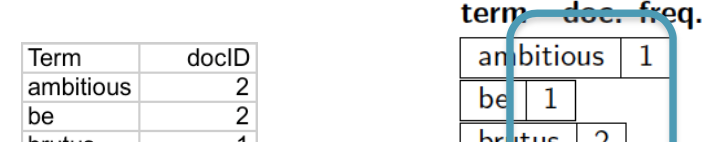
\includegraphics[height=1.5cm]{ir1}\\
Document frequency is number of times the term appear in different documents
\\
\\
\textbf{Boolean retrieval}\\
AND results in few results, OR results in many results, information overload!
\\
\textbf{Ranked retrieval}\\
query written in human language
\\
Rank each document with a score in [0, 1] which measures how well the document and query match
\\
\textbf{Bag of words}\\
doesn't consider ordering of words in document

\subsection*{Add one smoothing}
does not favor training data
\\
word with first letter capitalised is different from the word with first letter in lowercase
\\
double count add-one-smoothing maintains the counting separately, still add one but store the second count in another list
\\\\
\begin{equation*}
  \begin{aligned}
$\frac{\begin{array}{top} \textrm{ count\ of\ term\ in\ current\ corpus\ }+ \\
 \textrm{smoothed\ count\ of\ observed\ term}\end{array}}{\begin{array}{btm} \textrm{total\ counts\ for\ terms\ in\ doc\ for\ words\ in\ corpora }+\\ \textrm{total\ smoothed\ counts\ added\ for\ terms\ in\ corpora}\end{array}}}$
  \end{aligned}
\end{equation*}\\\\\\
% mixture model
This models rank documents that contains both terms higher than documents that contain less query terms\\
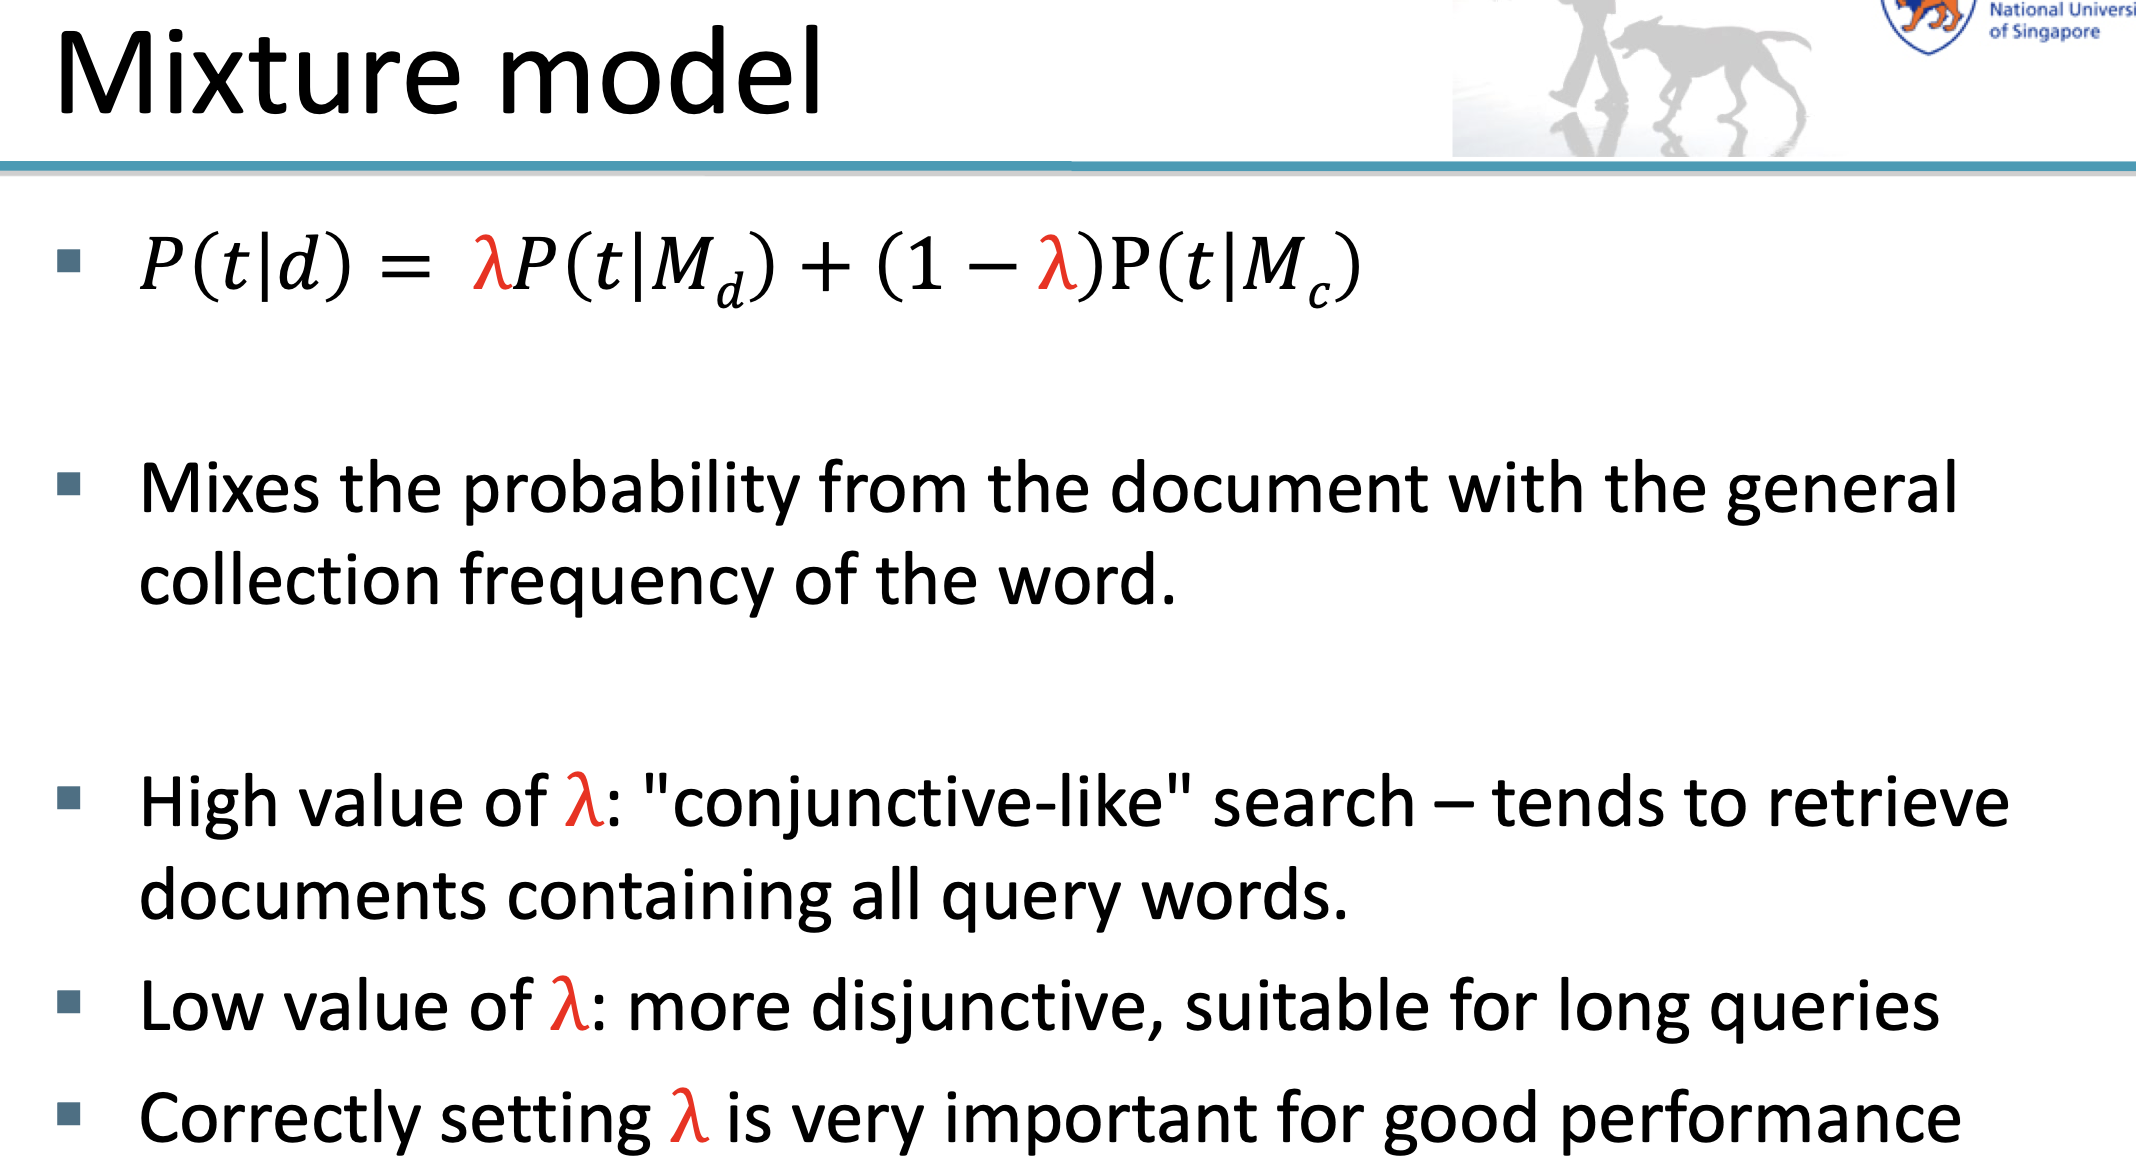
\includegraphics[height=5cm]{ir15}\\
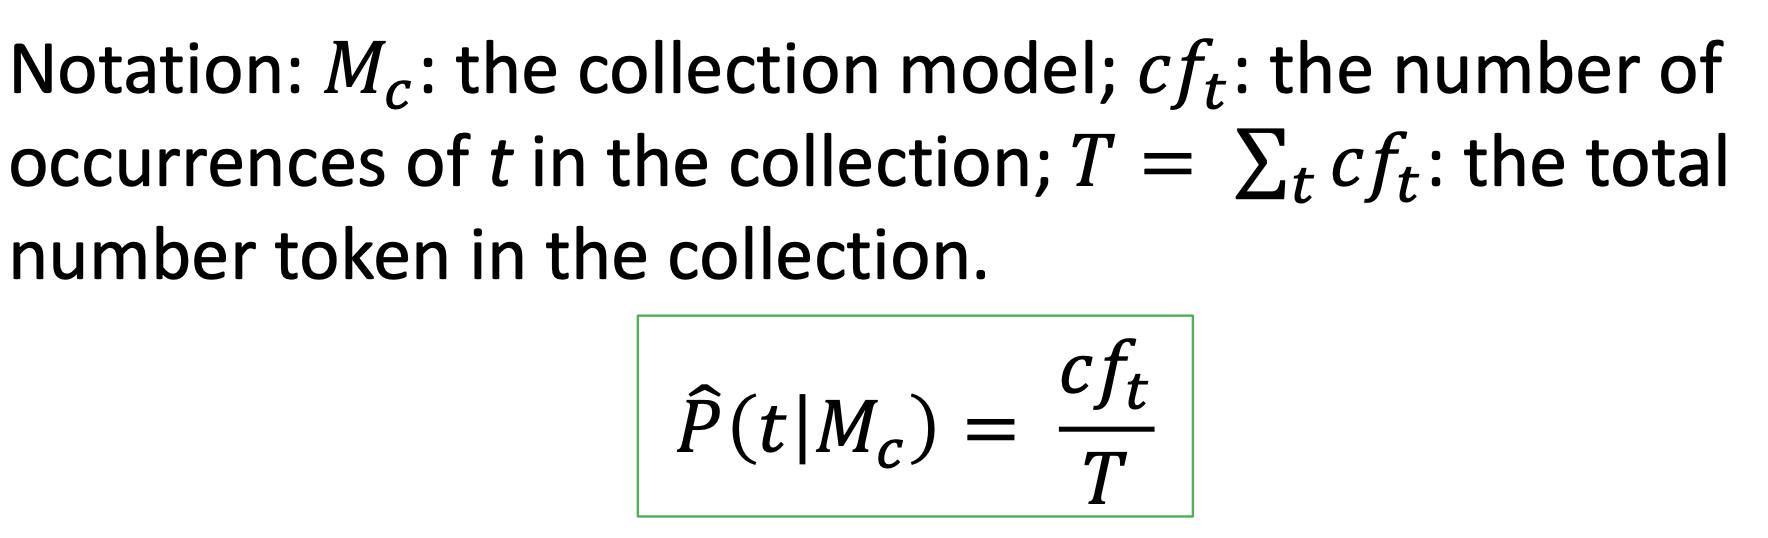
\includegraphics[height=2cm]{ir14}\\\\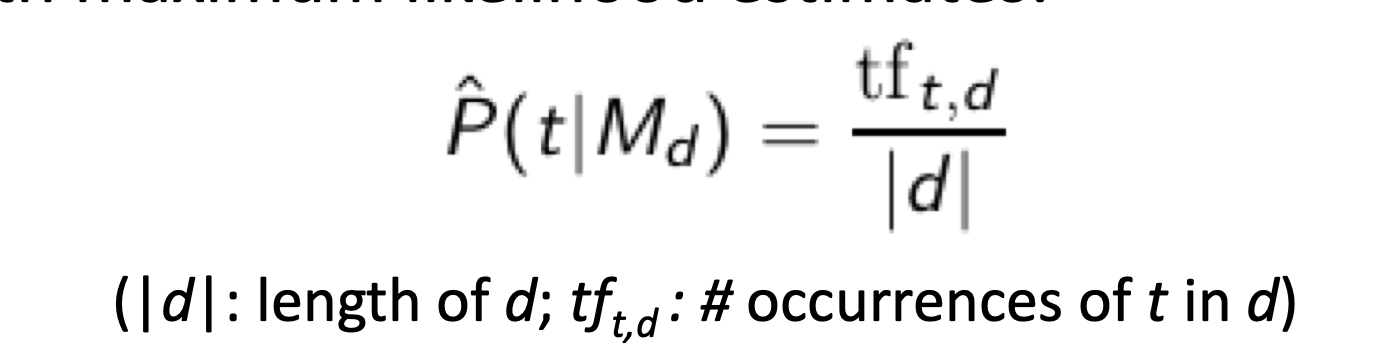
\includegraphics[height=1.5cm]{ir13}\\
\subsection*{Term count matrices}
Each document is a count (column) vector
\\
\subsection*{Language model}
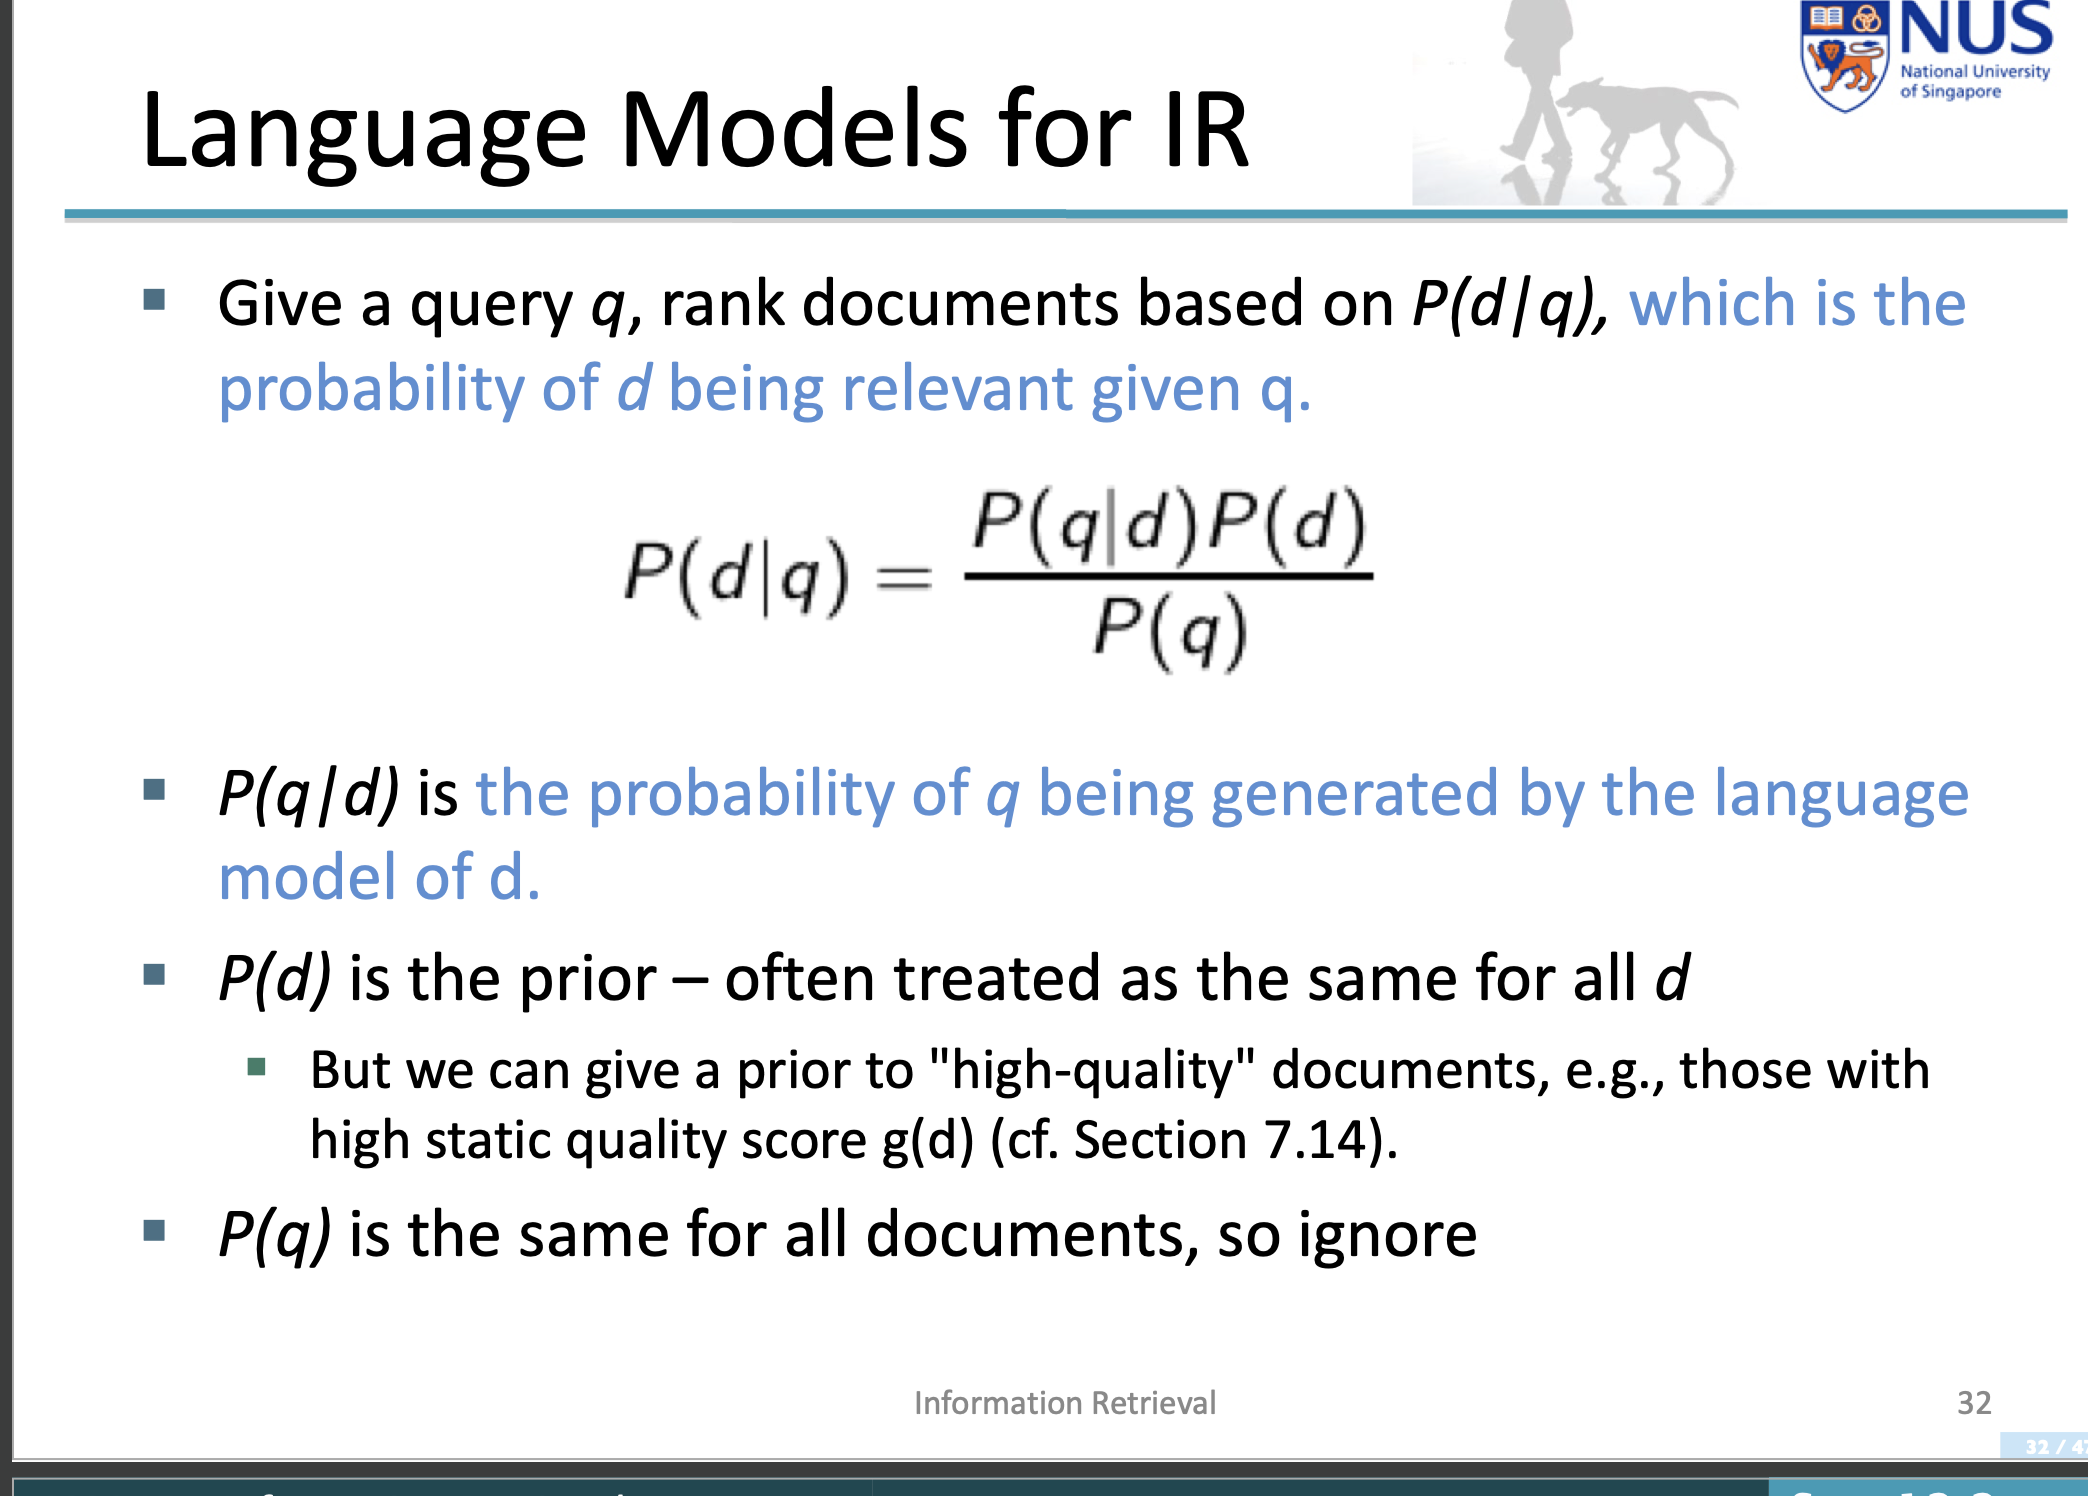
\includegraphics[height=5cm]{ir19}
\subsection*{tfxidf}
\textbf{tf weight} (log frequency) 1 + $log_{10}{tf}$ if tf $>$ 0 
\\\\
\textbf{inverse document frequency}
Meant to lower the weight of more common terms and increase weight for rare terms\\
$\mathrm{log_{10}{(collection\ size / df_{t}})}$
\\
\\
score will contain the weights for all terms in the q $\cap$ d
\subsection*{cosine similarity}
sum(q_{i} \ast d_{i})\\\\
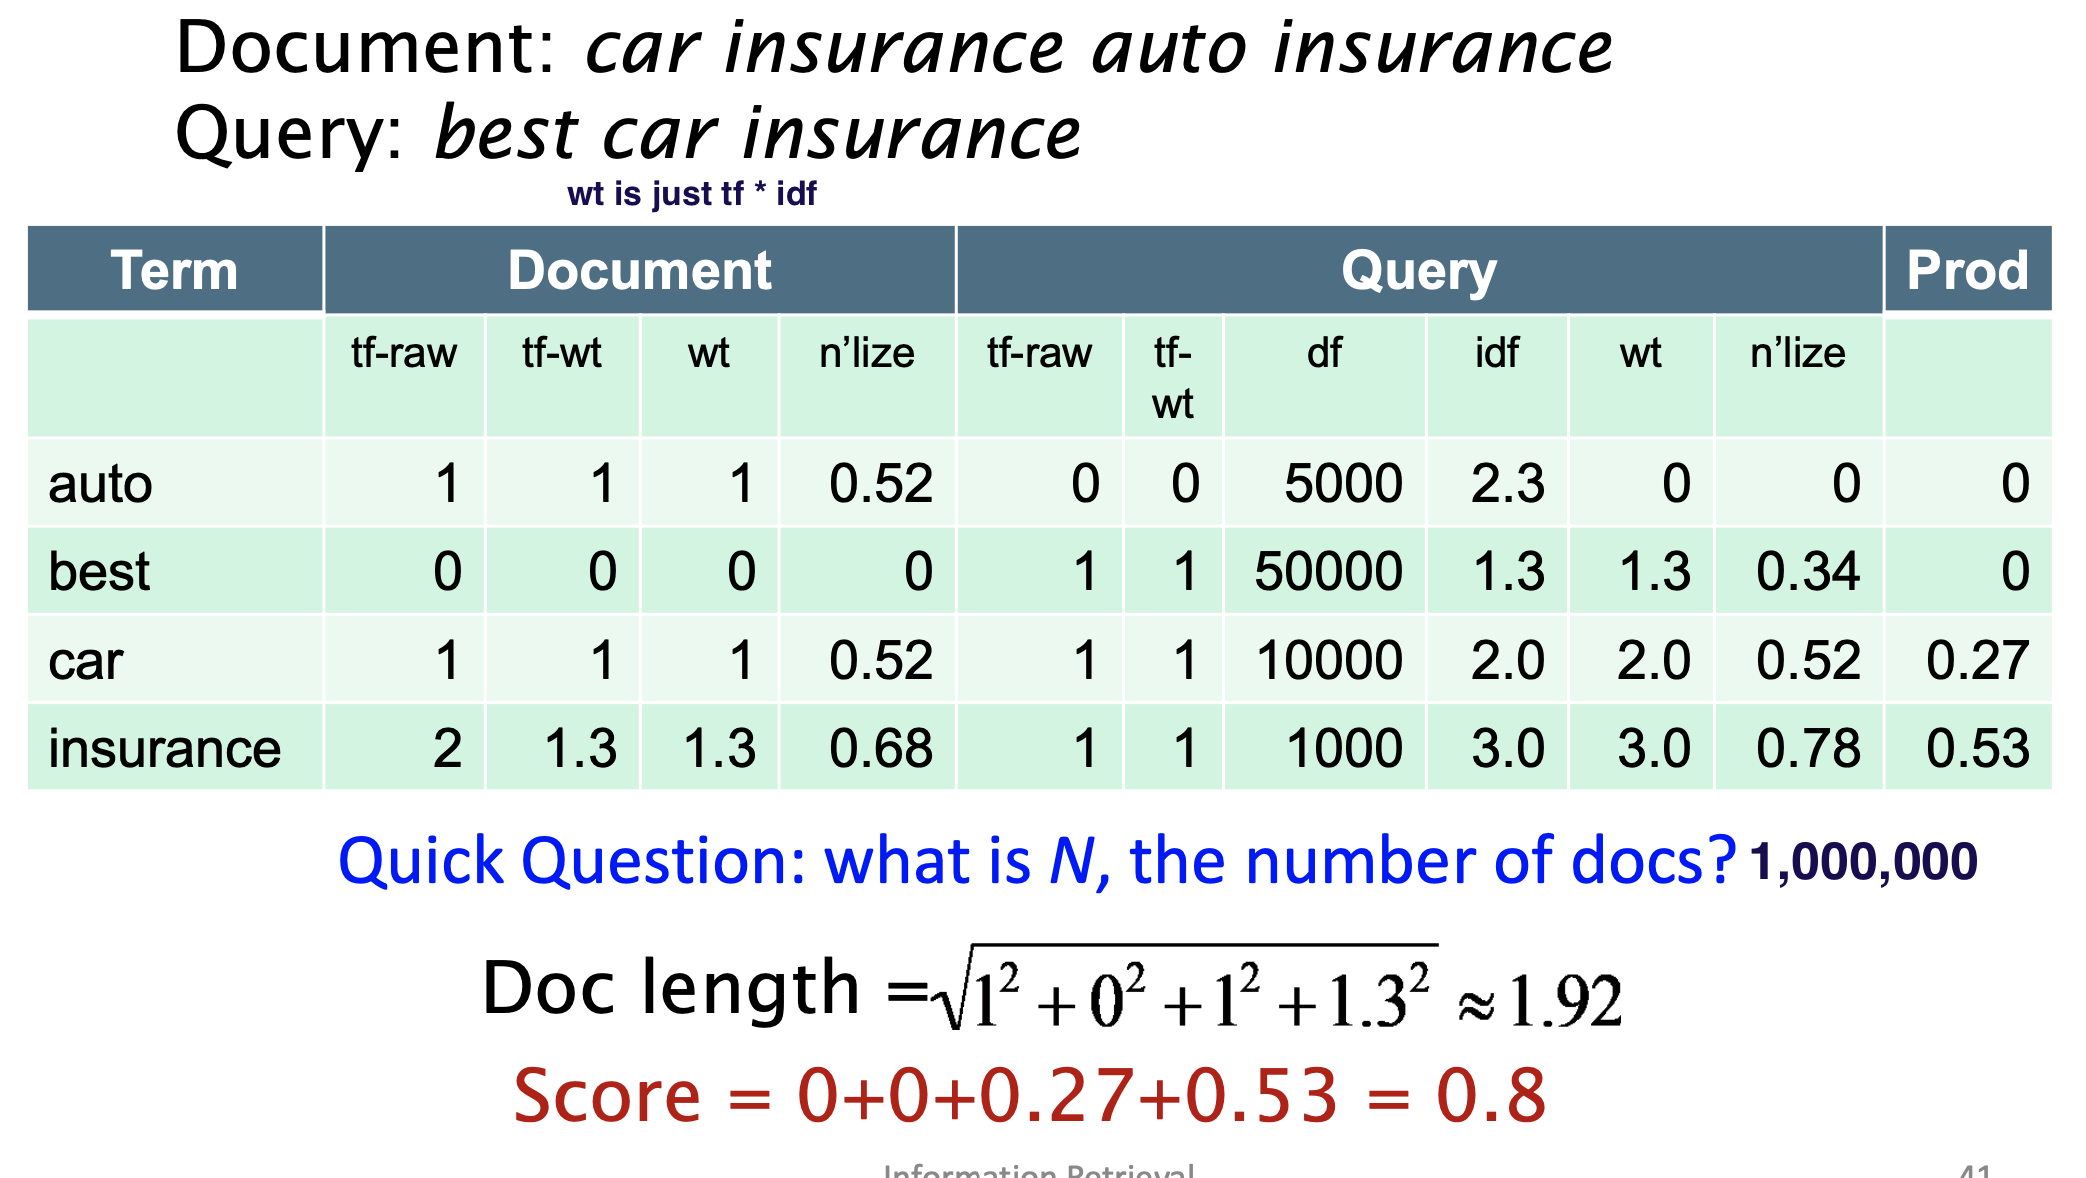
\includegraphics[height=5cm]{irl}
\subsection*{Biword index}
quiet phone call\\
2-gram\\
quiet phone, phone call
\\
False positives\\
but quiet phone can phone call may exist in different positions in the document 
False negatives cannot occur as it appears in posting list of "quiet phone" and "phone call"
and will be part of the intersection when merged and returned
\subsection*{Positional index}
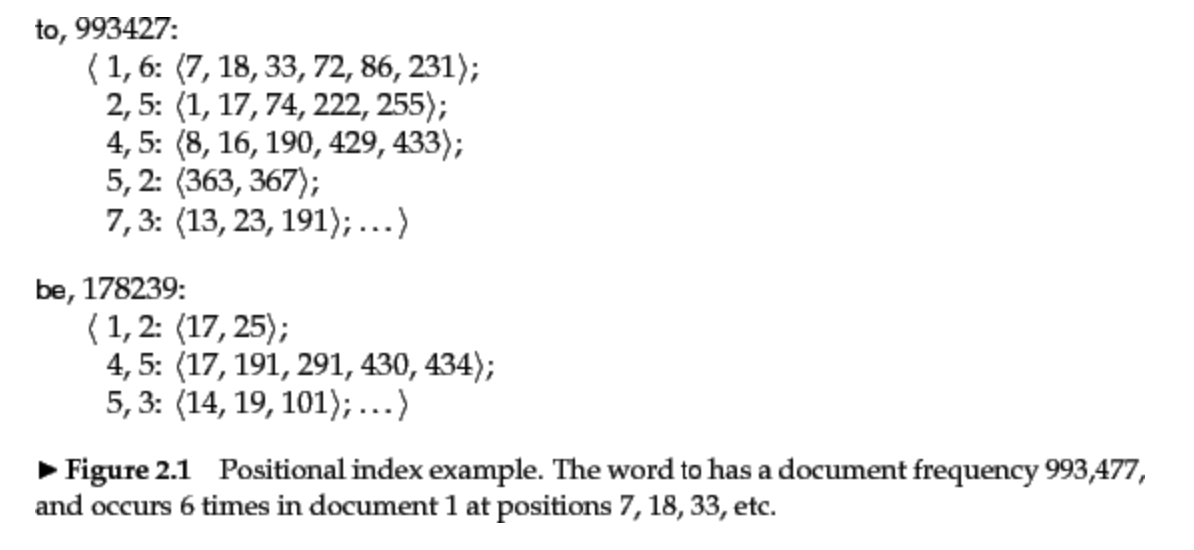
\includegraphics[height=3cm]{ir5}\\
narrow down the potential documents quickly \\
this is especially helpful when two juxtaposed query terms exist in many documents but whose intersection is small
\subsection*{Biword + Positional index}
A hybrid algorithm might first use the biword index to quickly determine the set of documents that could contain the query.
get $d_{to} \cap d_{be} $\\
Since doc 1 contains be 2 times, process doc 1\\\\
 Next, the algorithm would verify which candidate documents actually contain the phrase by checking through the positional postings. In both phases, we can use the strategy to process smaller document frequency items first. For efficiency, the biword index could also maintain the document frequency and postings pointer for its individual words, to save the cost of the additional dictionary lookups that would be incurred otherwise. 
\subsection*{Skip pointer}
skip pointer to point to end of list\\
10\\
$1 \rightarrow 2 \rightarrow 3 \rightarrow 4 \rightarrow 5$
\\\\
Dense cluster chance of skipping is high, it would be more effective to have a single skip pointer 1 \rightarrow 15\\
\\
\subsection*{Overlap measure- Jaccard coefficient}
assign number between 0 and 1
\\\\
$\frac{\| X \cap Y \|}{\| X \cup Y \| }$\\\\
for trigram Tue,ues,esd,sda,day\\ 
If both words are same, jaccard is 1\\
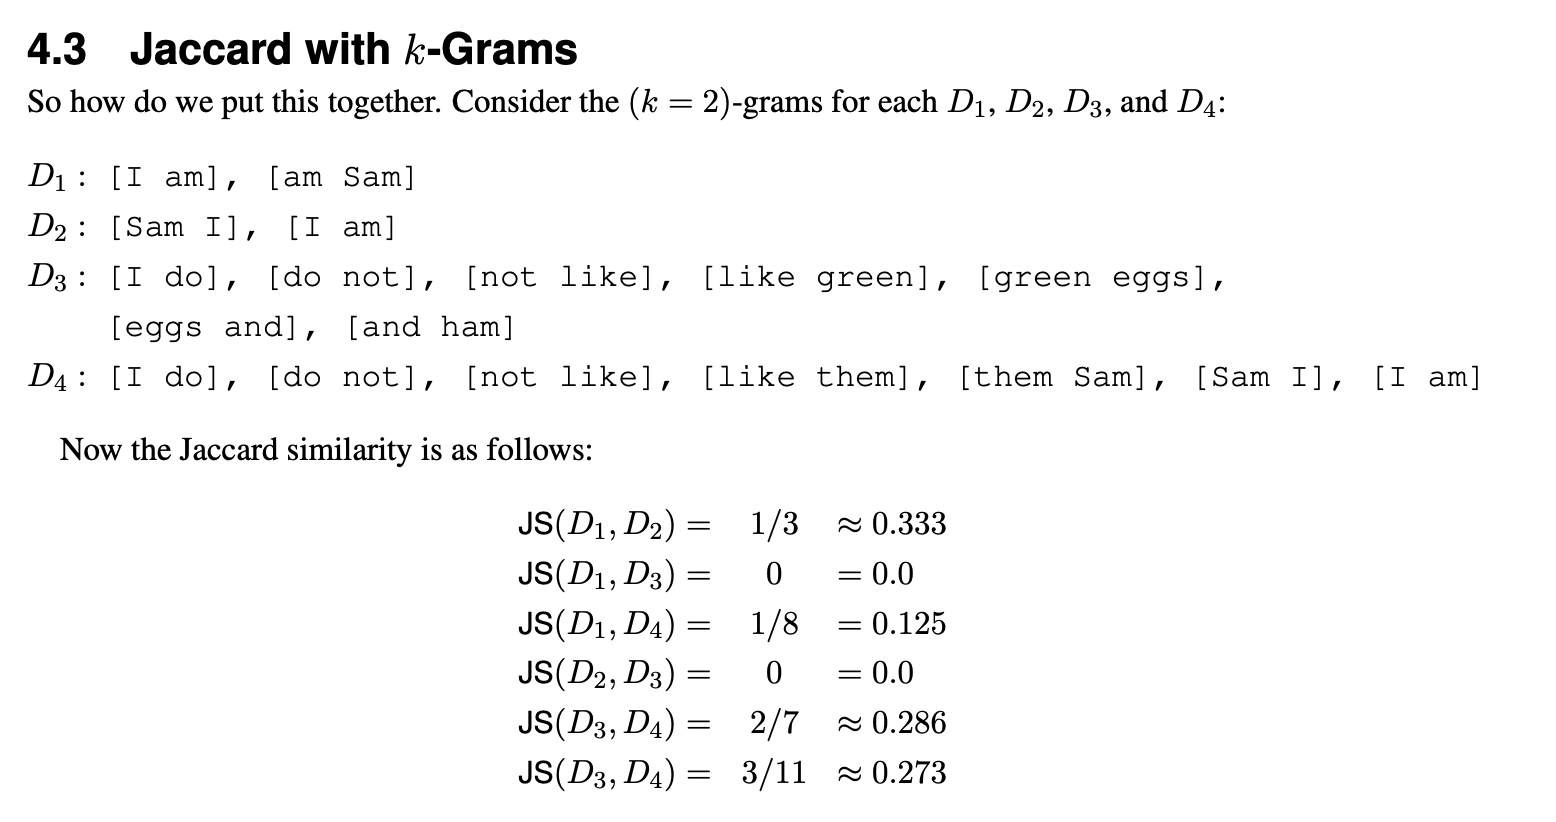
\includegraphics[height=5cm]{ir4}\\
\subsection*{Soundex}
only suitable for context of English\\
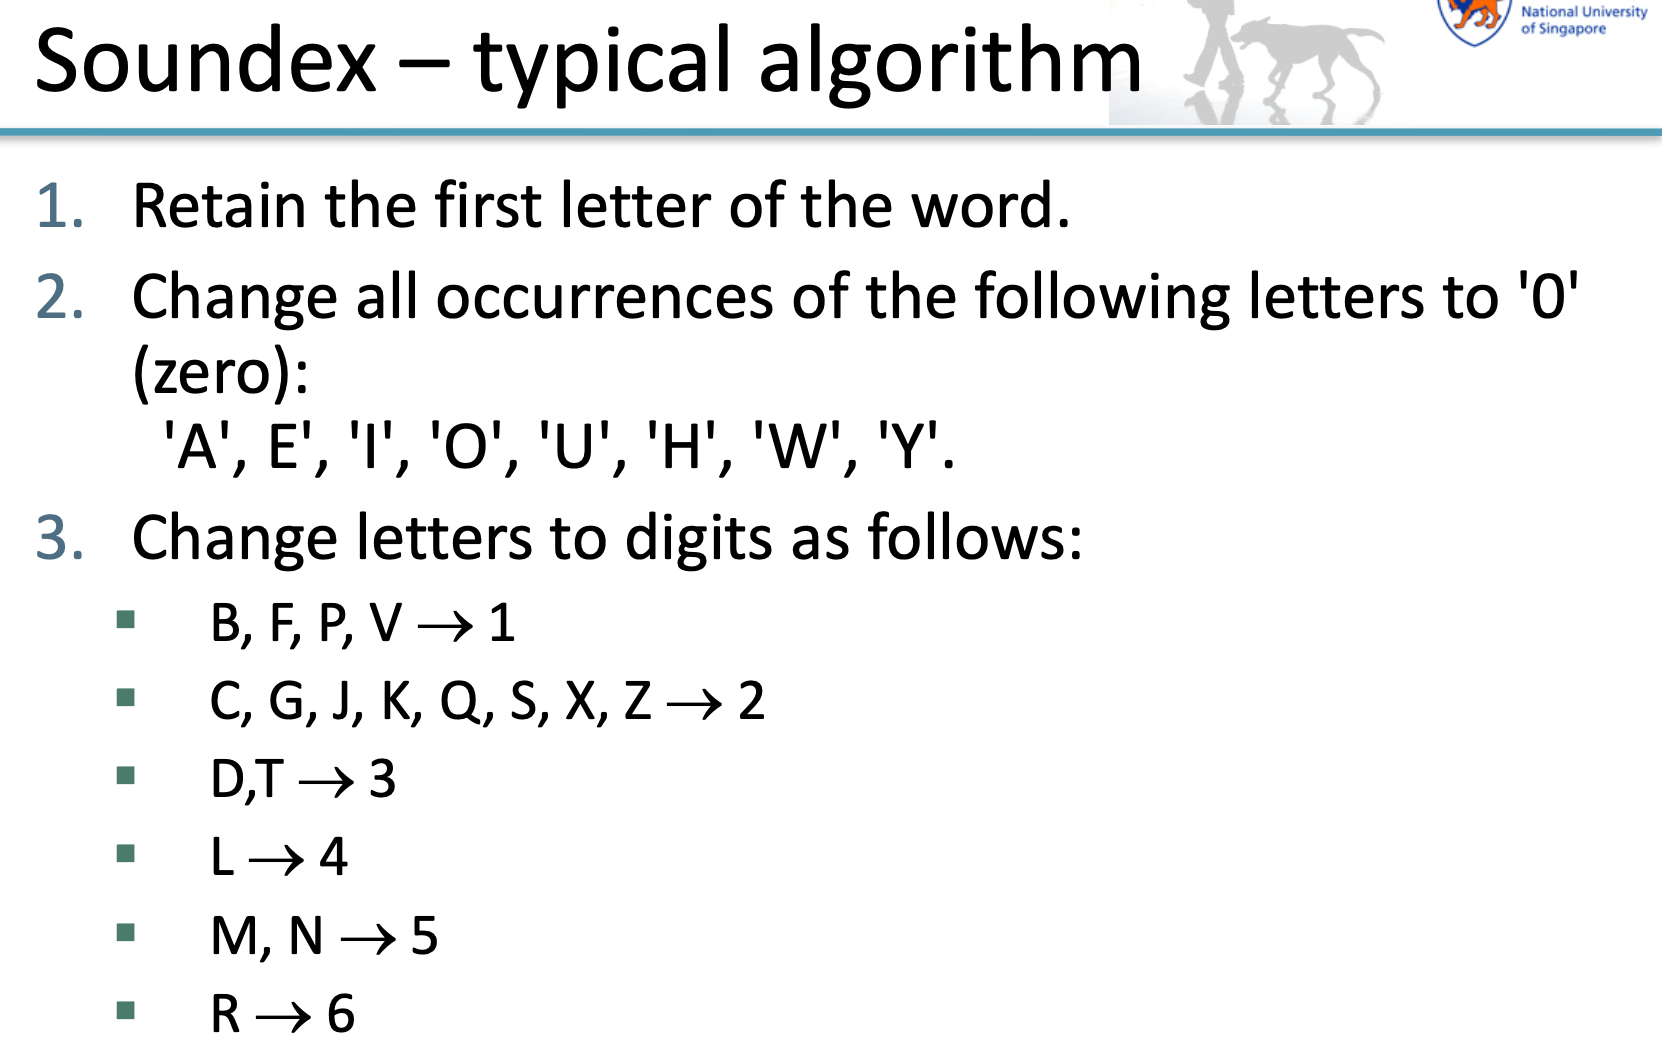
\includegraphics[height=5cm]{ir2}\\
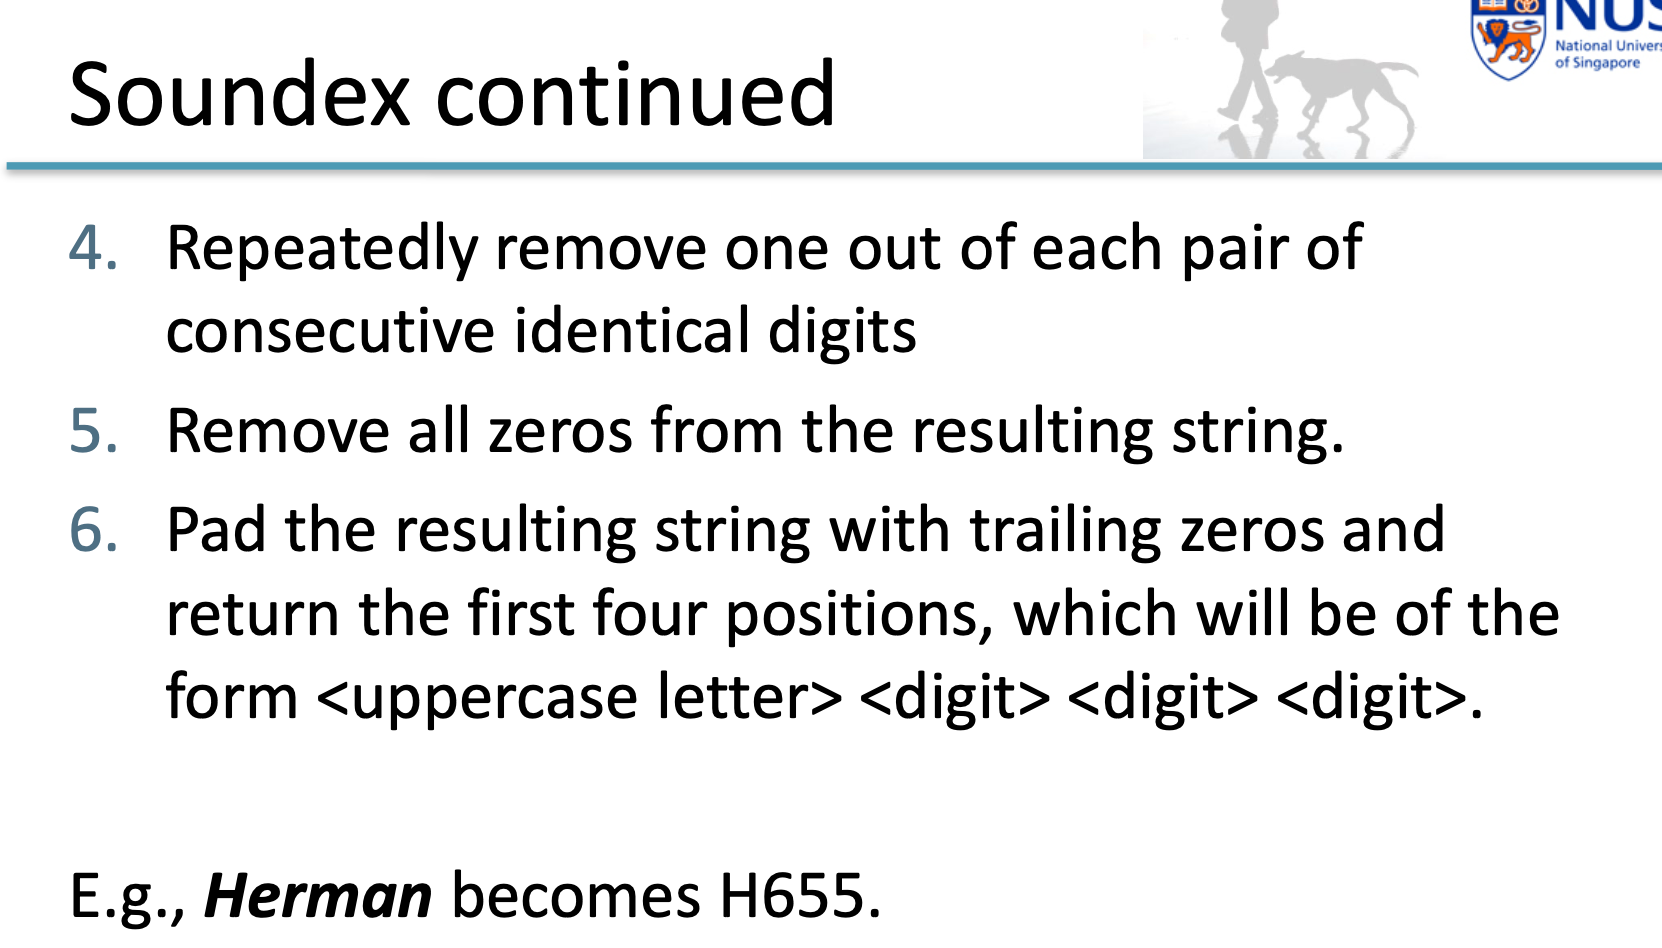
\includegraphics[height=5cm]{ir3}\\
\subsection*{Stop words removal}
cause some phrase search to be less precise
\subsection*{Permuterm index}\\
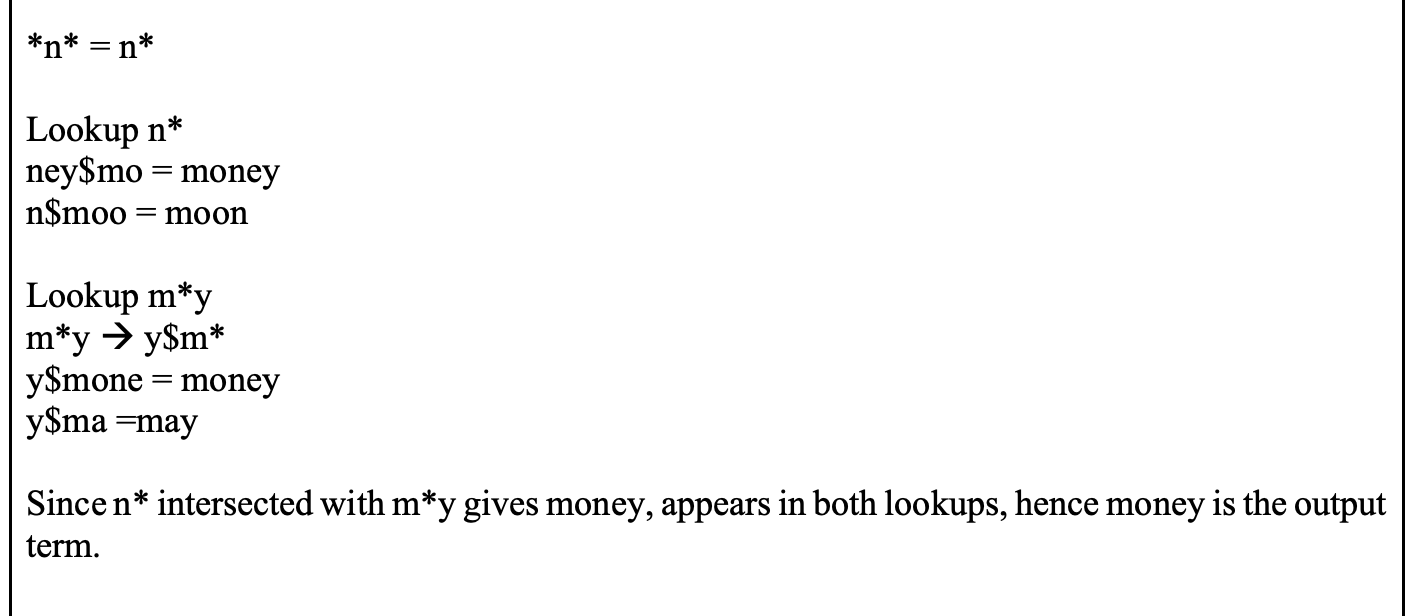
\includegraphics[height=5cm]{ir6}\\
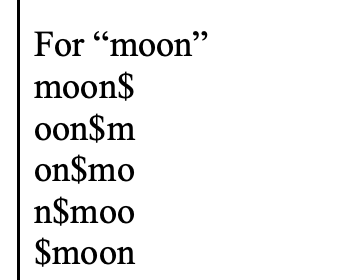
\includegraphics[height=2cm]{ir7}
\subsection*{Heuristics}
avoid unnecessary / time consuming computations\\
\textbf{Index elimination}\\
\textbf{Champion list - Tiered lists}\\
\textbf{Impact-ordered postings - Early termination}\\
sort by weight of the term frequency in the document\\
because not sorted by document id, cannot find the intersection\\
terminate when a fixed number or below a wf threshold (e.g. threshold 0.5, anything lower will not be included)\\
take the union as there's no concurrent traversal\\\\
\textbf{Cluster pruning}\\
leaders are chosen at random, and followers are precomputed\\\\
a document will be the follower of the leader whose cosine similarity with the document is the highest\\\\
Note: When computing cos similarity between docs, all the terms have to be considered not just the query\\\\
Only need to rank the documents in one cluster
\subsection*{Measure of search engine}
Accuracy = (tp + tn) / (tp + fp + tn + fn)\\\\
Combined measure F\\
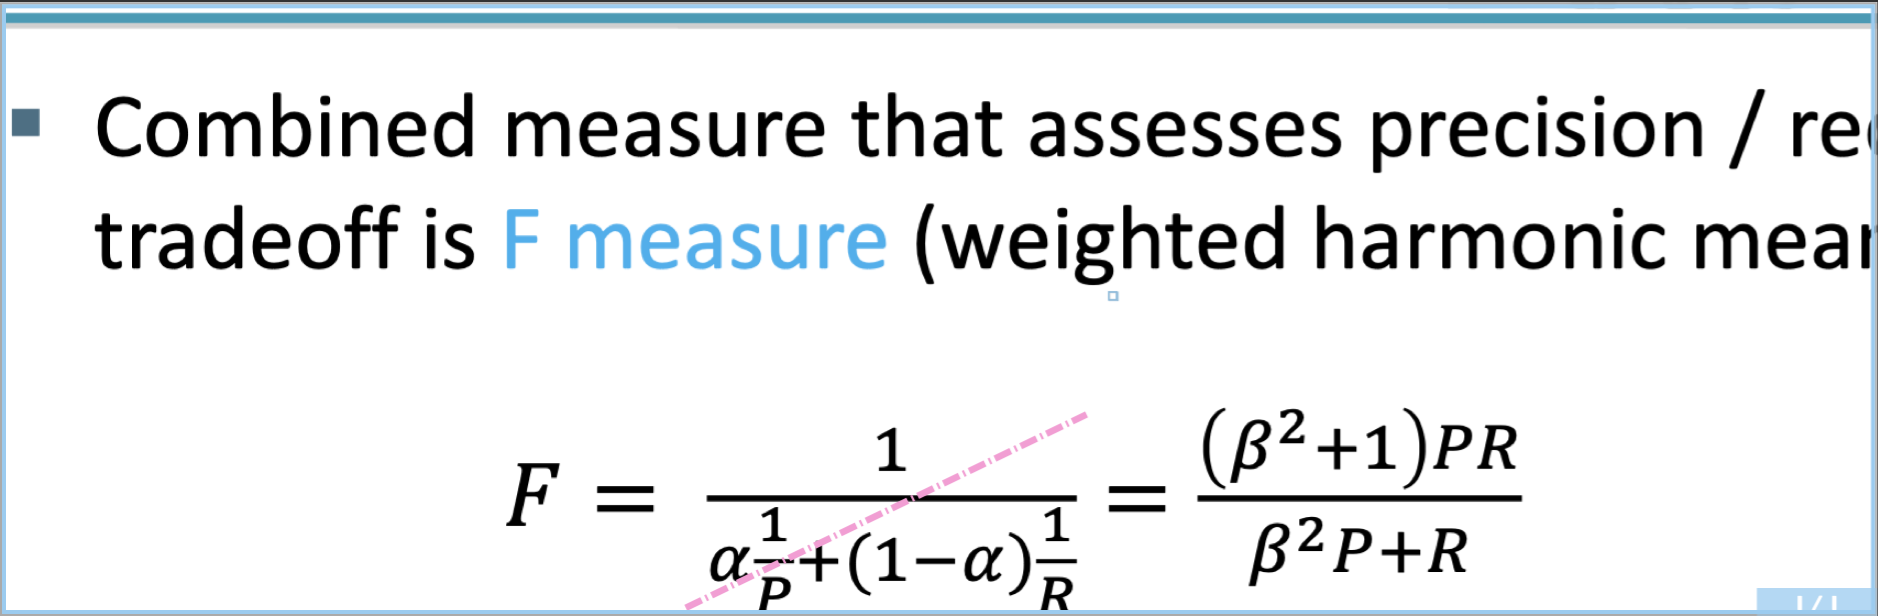
\includegraphics[height=3cm]{ir8}\\
Harmonic mean, balanced \\
$\frac{2PR}{P + R}$\\\\
P = $\mathrm{\frac{relevant\ documents\ retrieved}{retrieved\ documents}}$\\\\
R = $\mathrm{\frac{relevant\ documents\ retrieved}{relevant\ documents}}$\\
\\
\textbf{Interpolated precision}\\
Low point (ignore the drastic drop) does not reflect actual performance because it is going to go up later\\
Take the highest possible precision from the right\\
\\
How to know if the doc is relevant?\\
Boolean search engine, if document contains most words in the query\\
\textbf{Evaluate ranked results}\\
For all the relevant documents add (P, R)\\
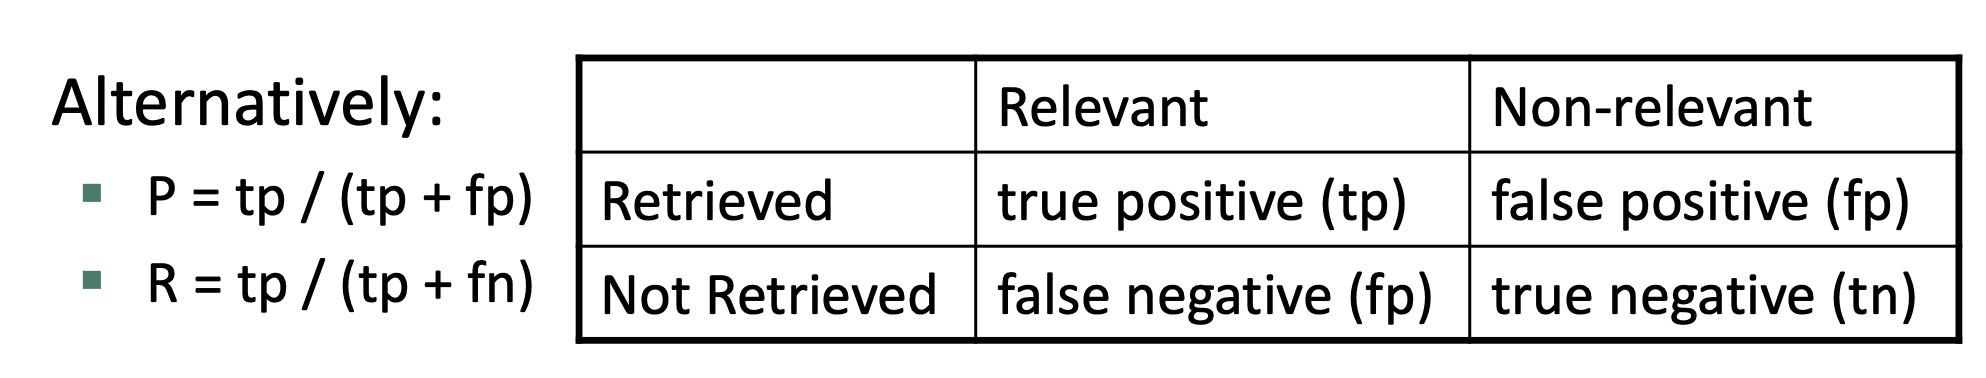
\includegraphics[height=2cm]{ir9}
\subsection*{Kappa measure}
Eliminate the factor agreement of chance\\
\)\)\)
P(A) = (relevant docs $|$ agree + nr docs $|$ agree) / $\#$docs = 0.925\\
P(non-relevant) = $\mathrm{\frac{judge\#1\ says\ non-relevant\ + judge\#2\ says\ non-relevant\ }{\# docs\ \ast\ 2\ }}$\\
P(E) = $P(\textrm{non relevant})^{2} + P(\textrm{relevant})^{2}$\\
Kappa (K) = [P(A)-P(E)]/[1-P(E)]\\
 Kappa $>$ 0.8 Good agreement\\
0.67 $<$ Kappa $<$ 0.8 Tentative conclusions\\
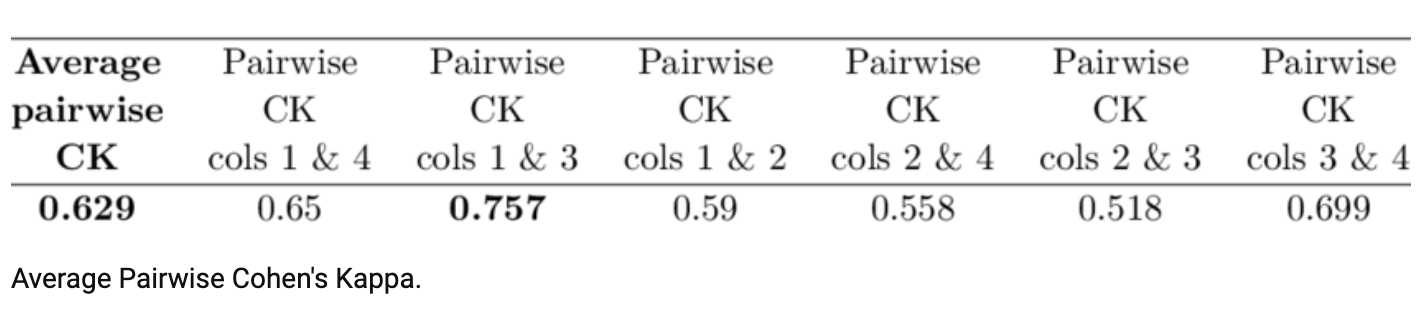
\includegraphics[height=2cm]{ir10}
\subsection*{Query refinement}\\
\textbf{Document level}\\
Standard RF Explicit feedback\\
Pseudo RF Explicit RF no feedback- Rocchio\\
RF does not work if there are misspellings/ mismatch
\\
Blind feedback assumes that top k is actually relevant\\
\textbf{Term level}\\
Manual thesaurus
\subsection*{To cut down index size}
Remove stop words 200MB savings\\
VB encoding during SPIMI block splitting stage 400MB savings\\
remove CSS/JS/HTML/Chinese characters, terms with only punctuations
posting compression (gap encoding)\\\\
\textbf{Posting compression -Variable byte (VB) coding}\\
Last byte continuation bit is 1\\
To get the original number, remove the continuation bit and combine\\
Posting stored as, start number byte + gap byte...\\
0A and 1B, then the original bit represenation is AB\\\\
\textbf{Index compression without blocking}\\
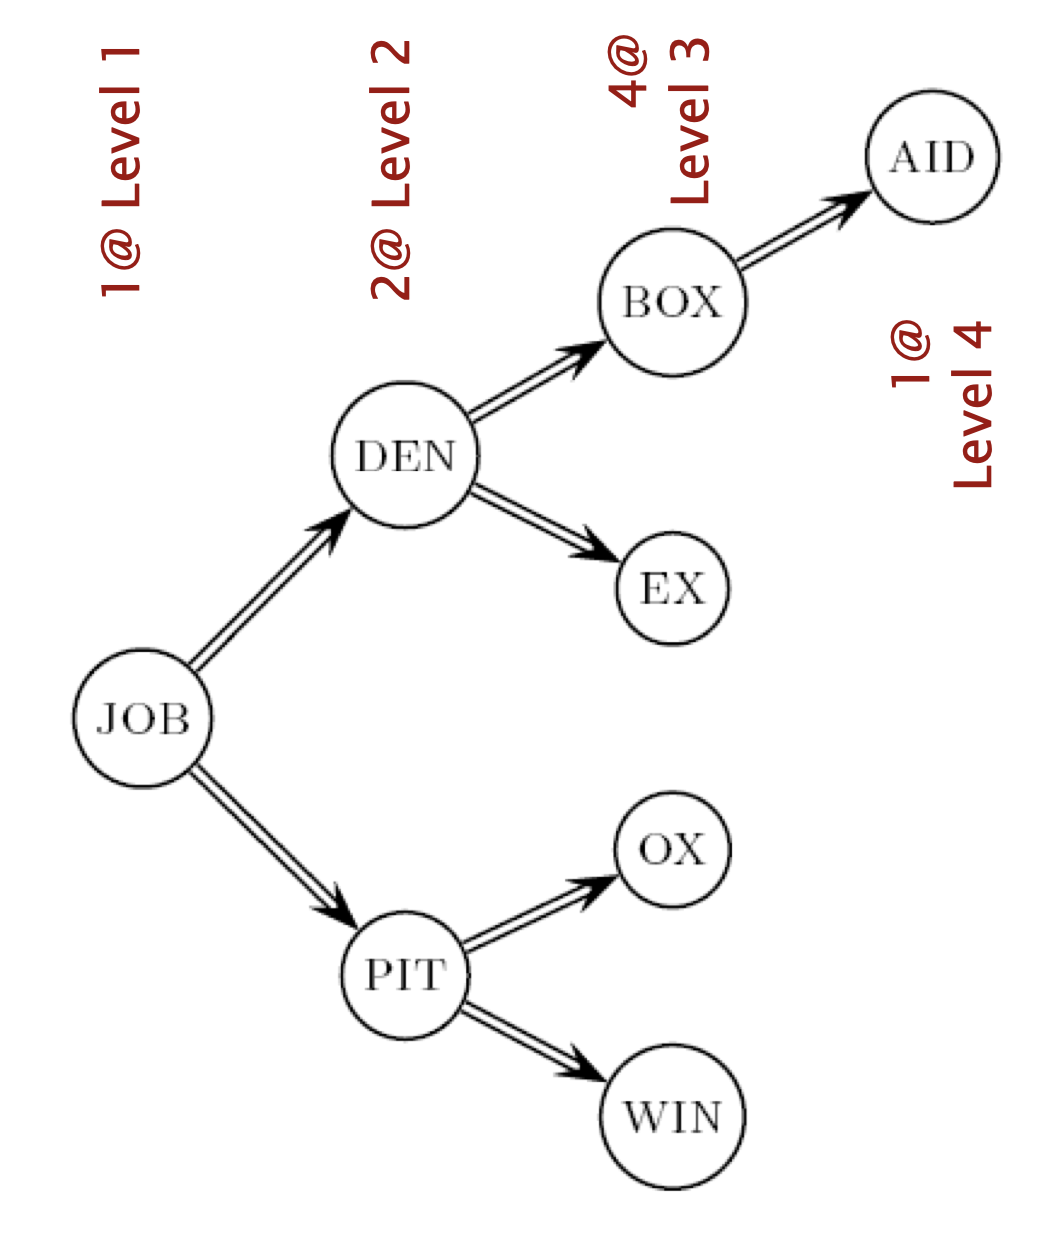
\includegraphics[height=3cm]{ir11}\\
level multiplied by \#nodes at the level\\
1 * 1 + 2 * 2 + 3 * 4 + 4 * 1\\\\
Takes 3 comparison to find the word EX \\\\
\textbf{Dictionary as a string}
terms 20 bytes\\
freq 4 bytes $\rightarrow$ store as pointer instead (1 byte)\\ 
postings ptr 4 bytes\\\\
\textbf{Index compression with blocking}\\
Linear search in k term block\\
if k = 4, construct block from Level 4
number of comparisons is going to increase\\
\# terms / block size = comparisons on each level\\\\
\textbf{Front coding}\\
Put the $\ast$ before the first letter that changes for all the cases\\
Number counted is for the entire word without $\ast$\\
\\
1◊ represents 1 character that follow after the diamond\\
Repeat the process for the current word\\
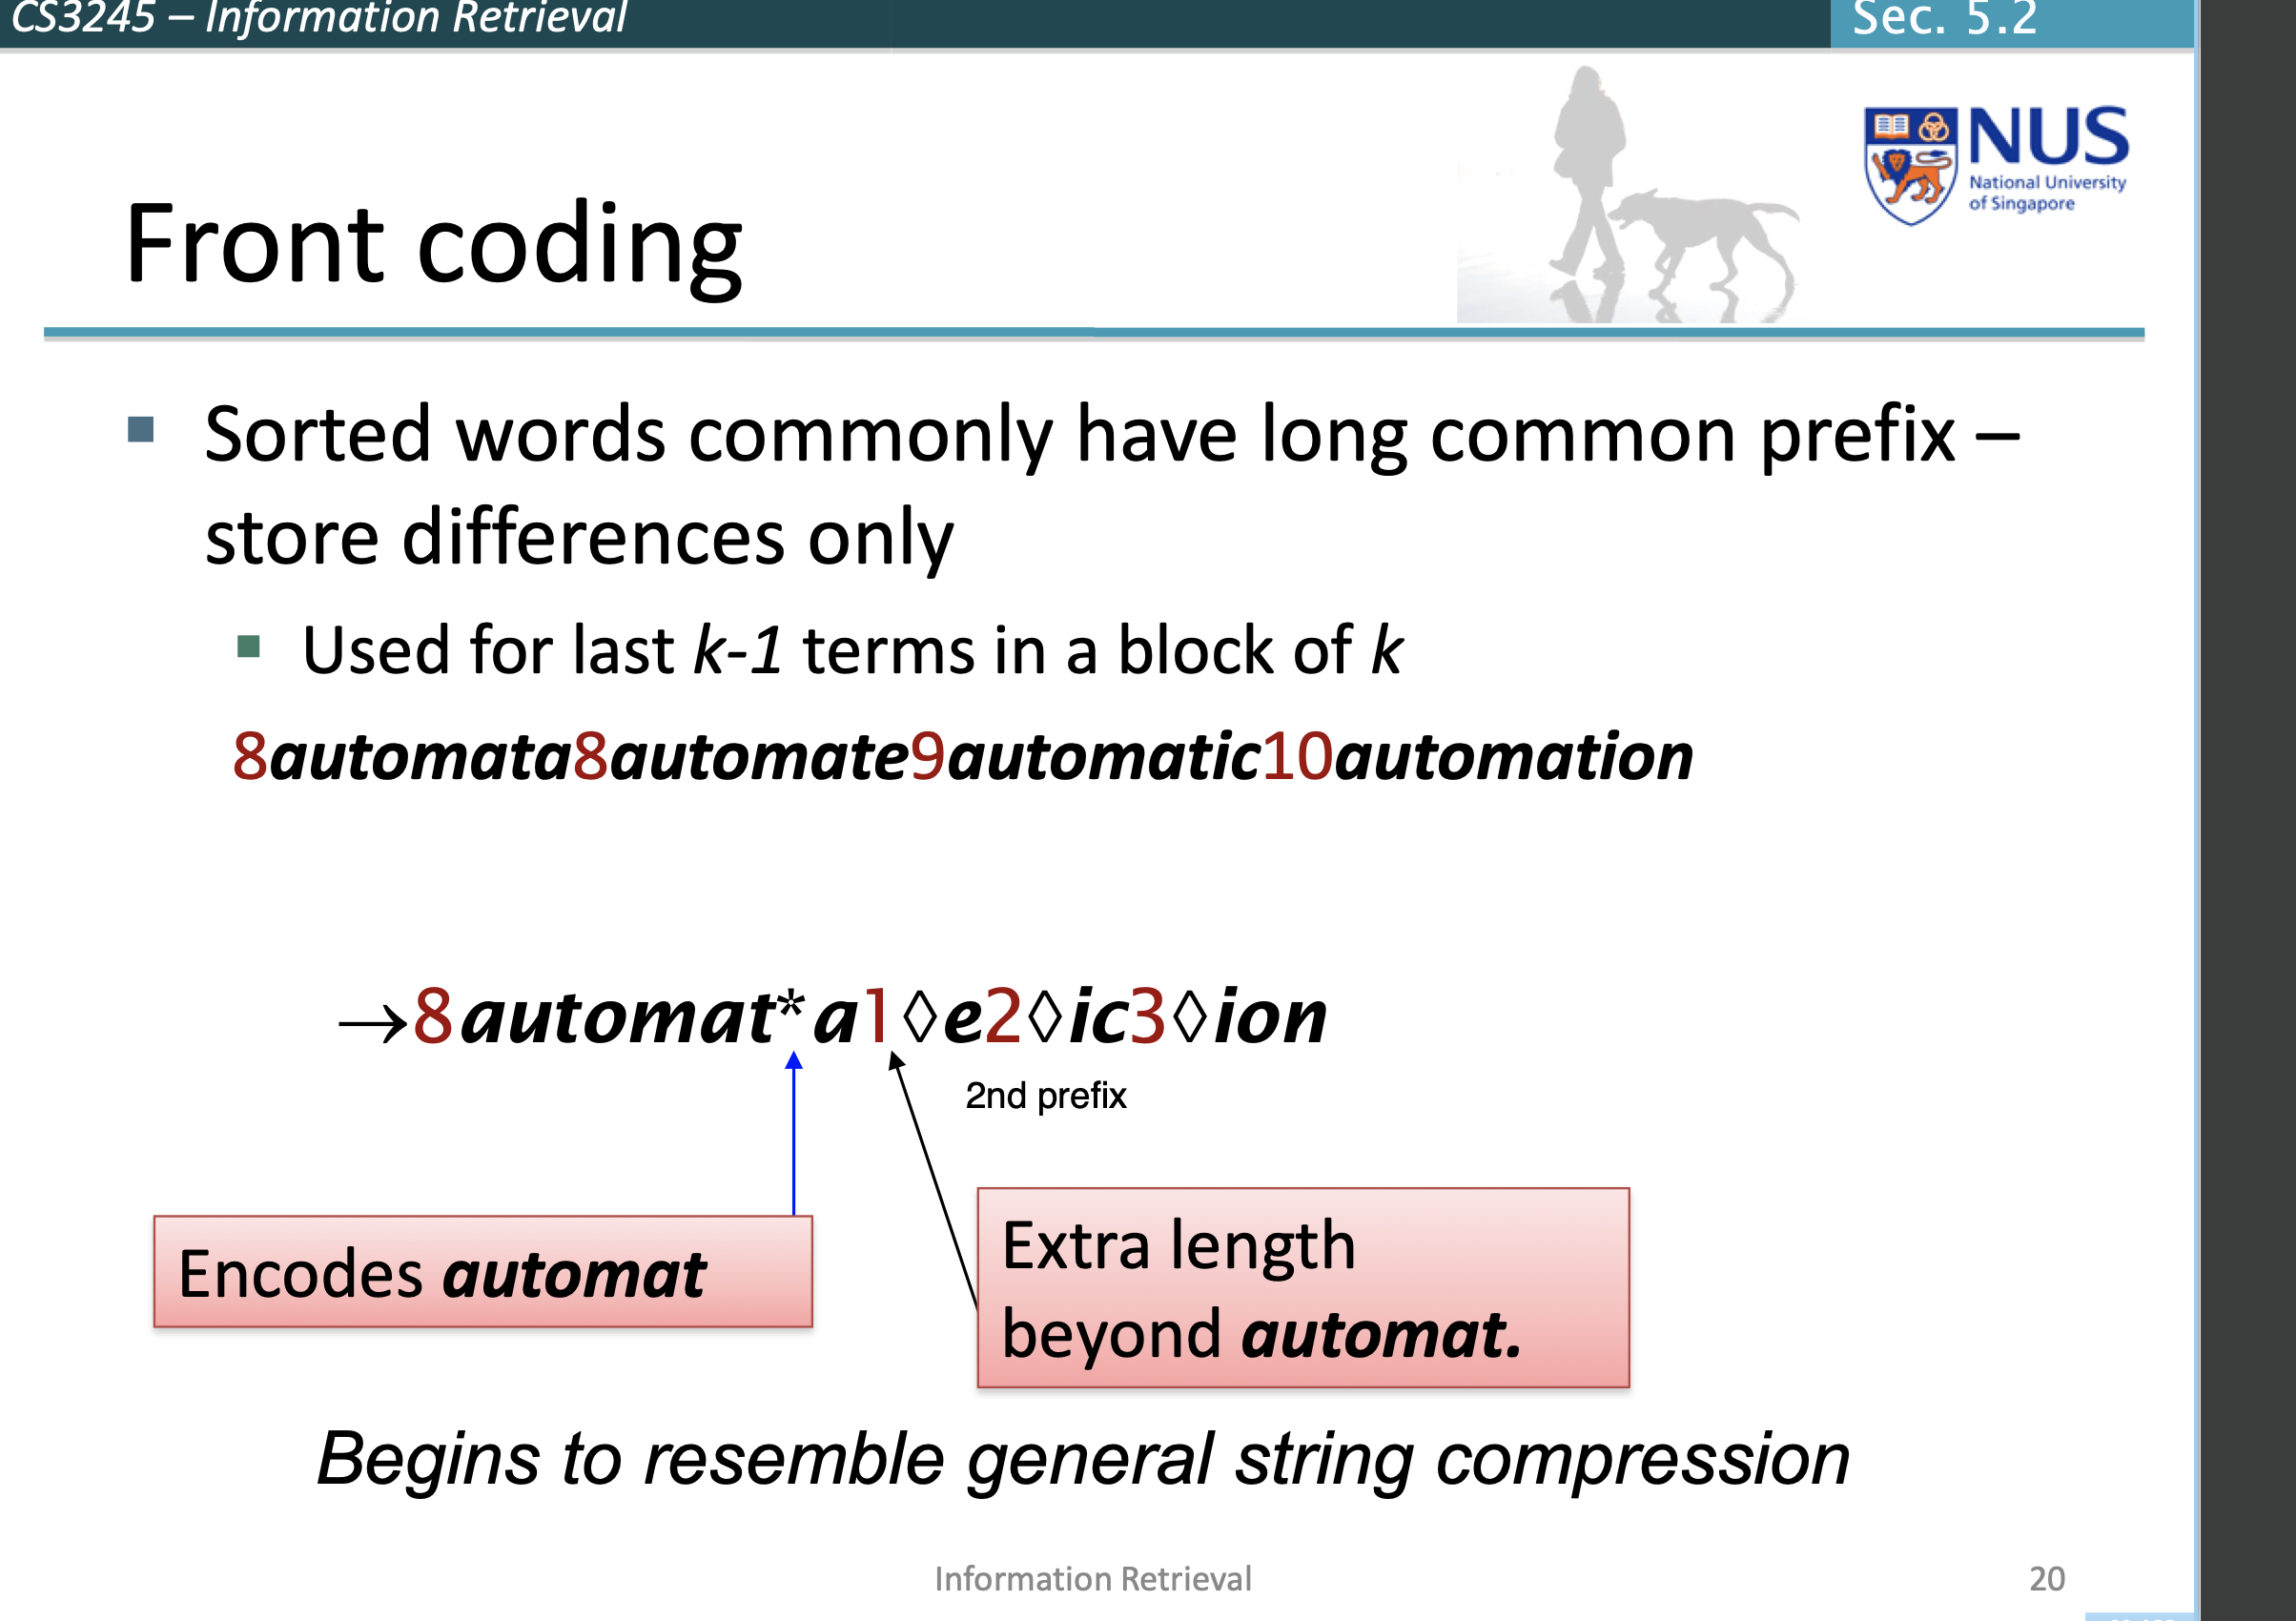
\includegraphics[height=5cm]{ir17}
\subsection*{XML retrieval}
Pseudo xpath /person/name#Bob\\
\textbf{Context resemblance}\\
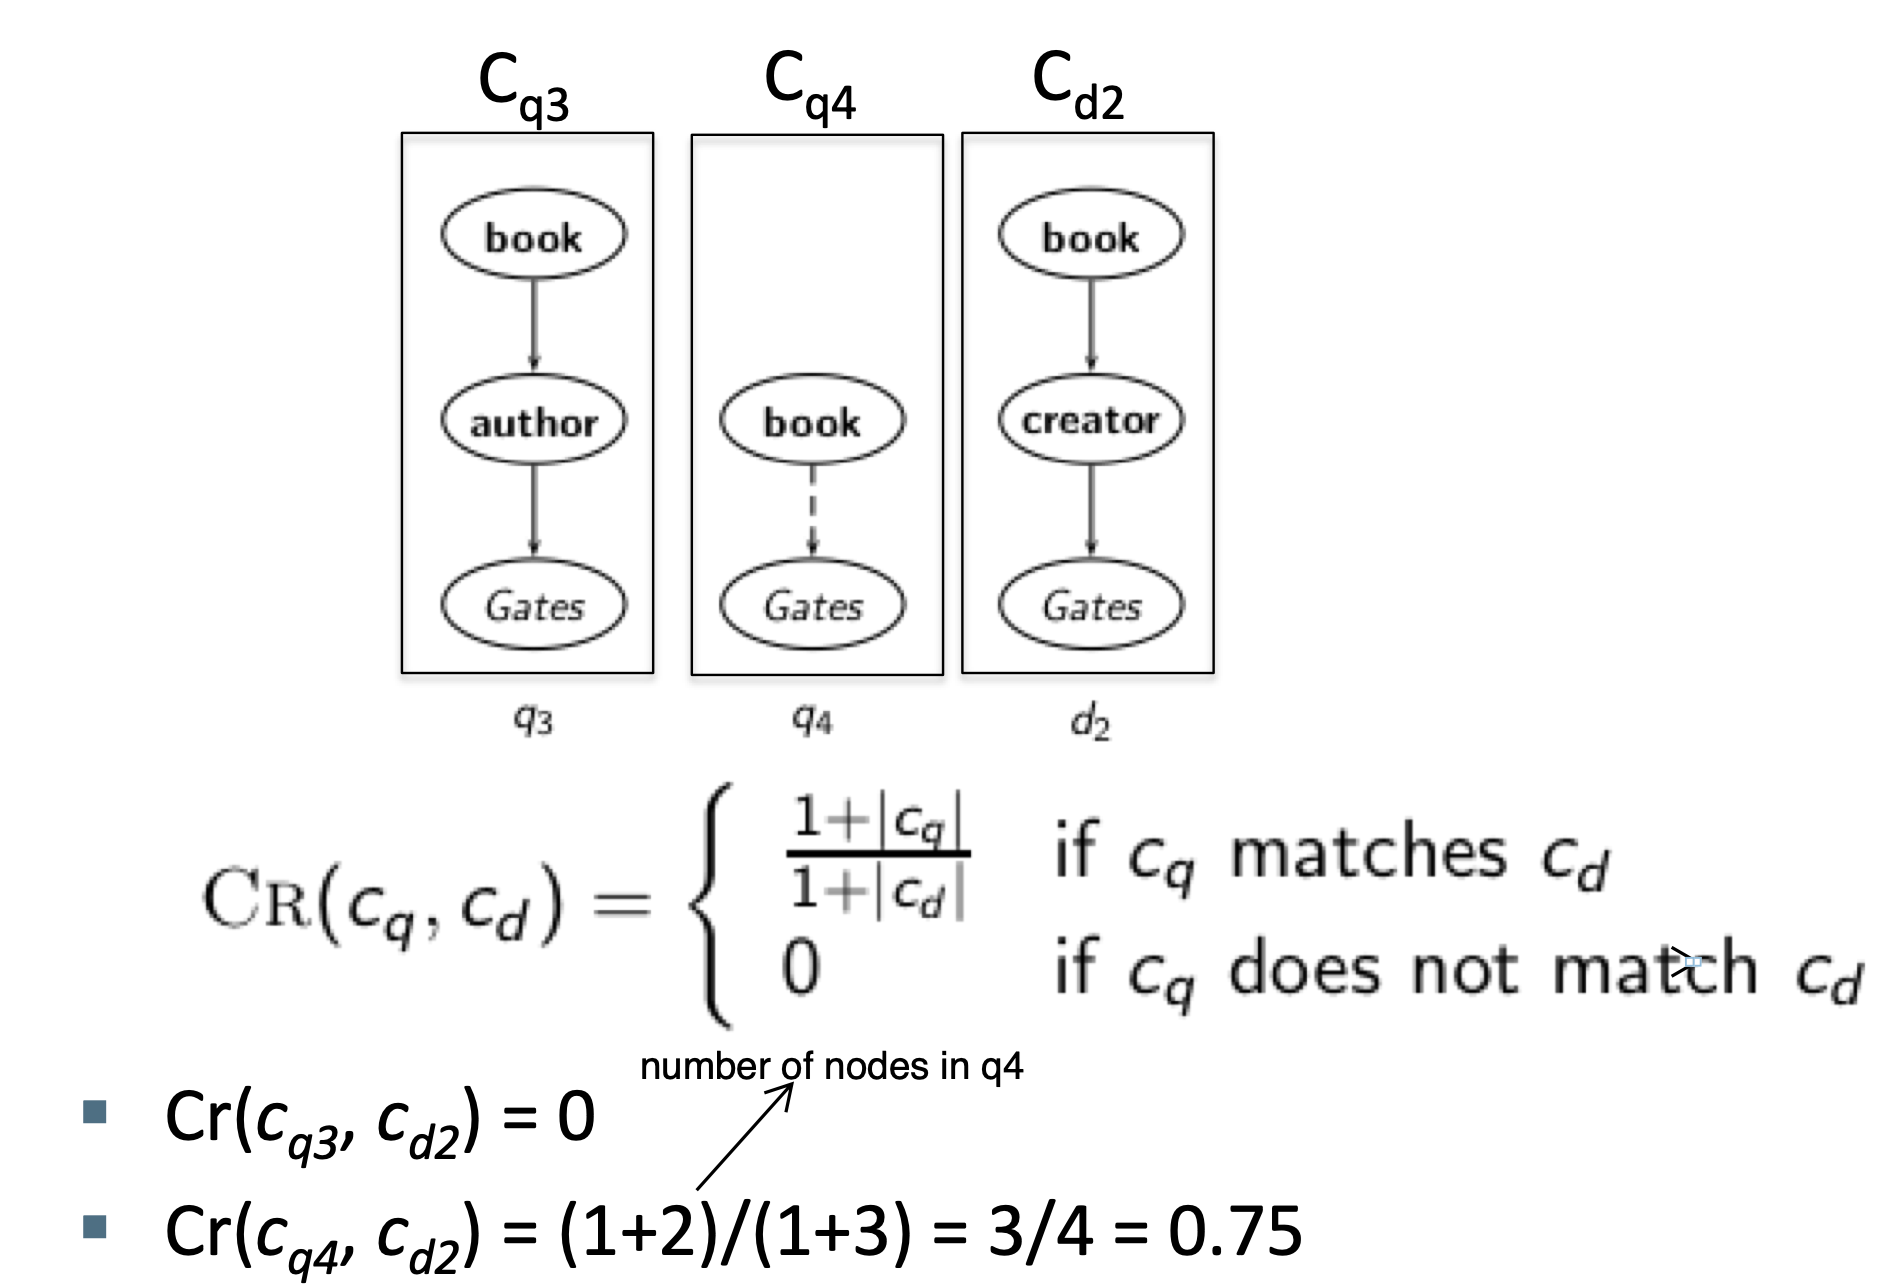
\includegraphics[height=3cm]{ir12}\\
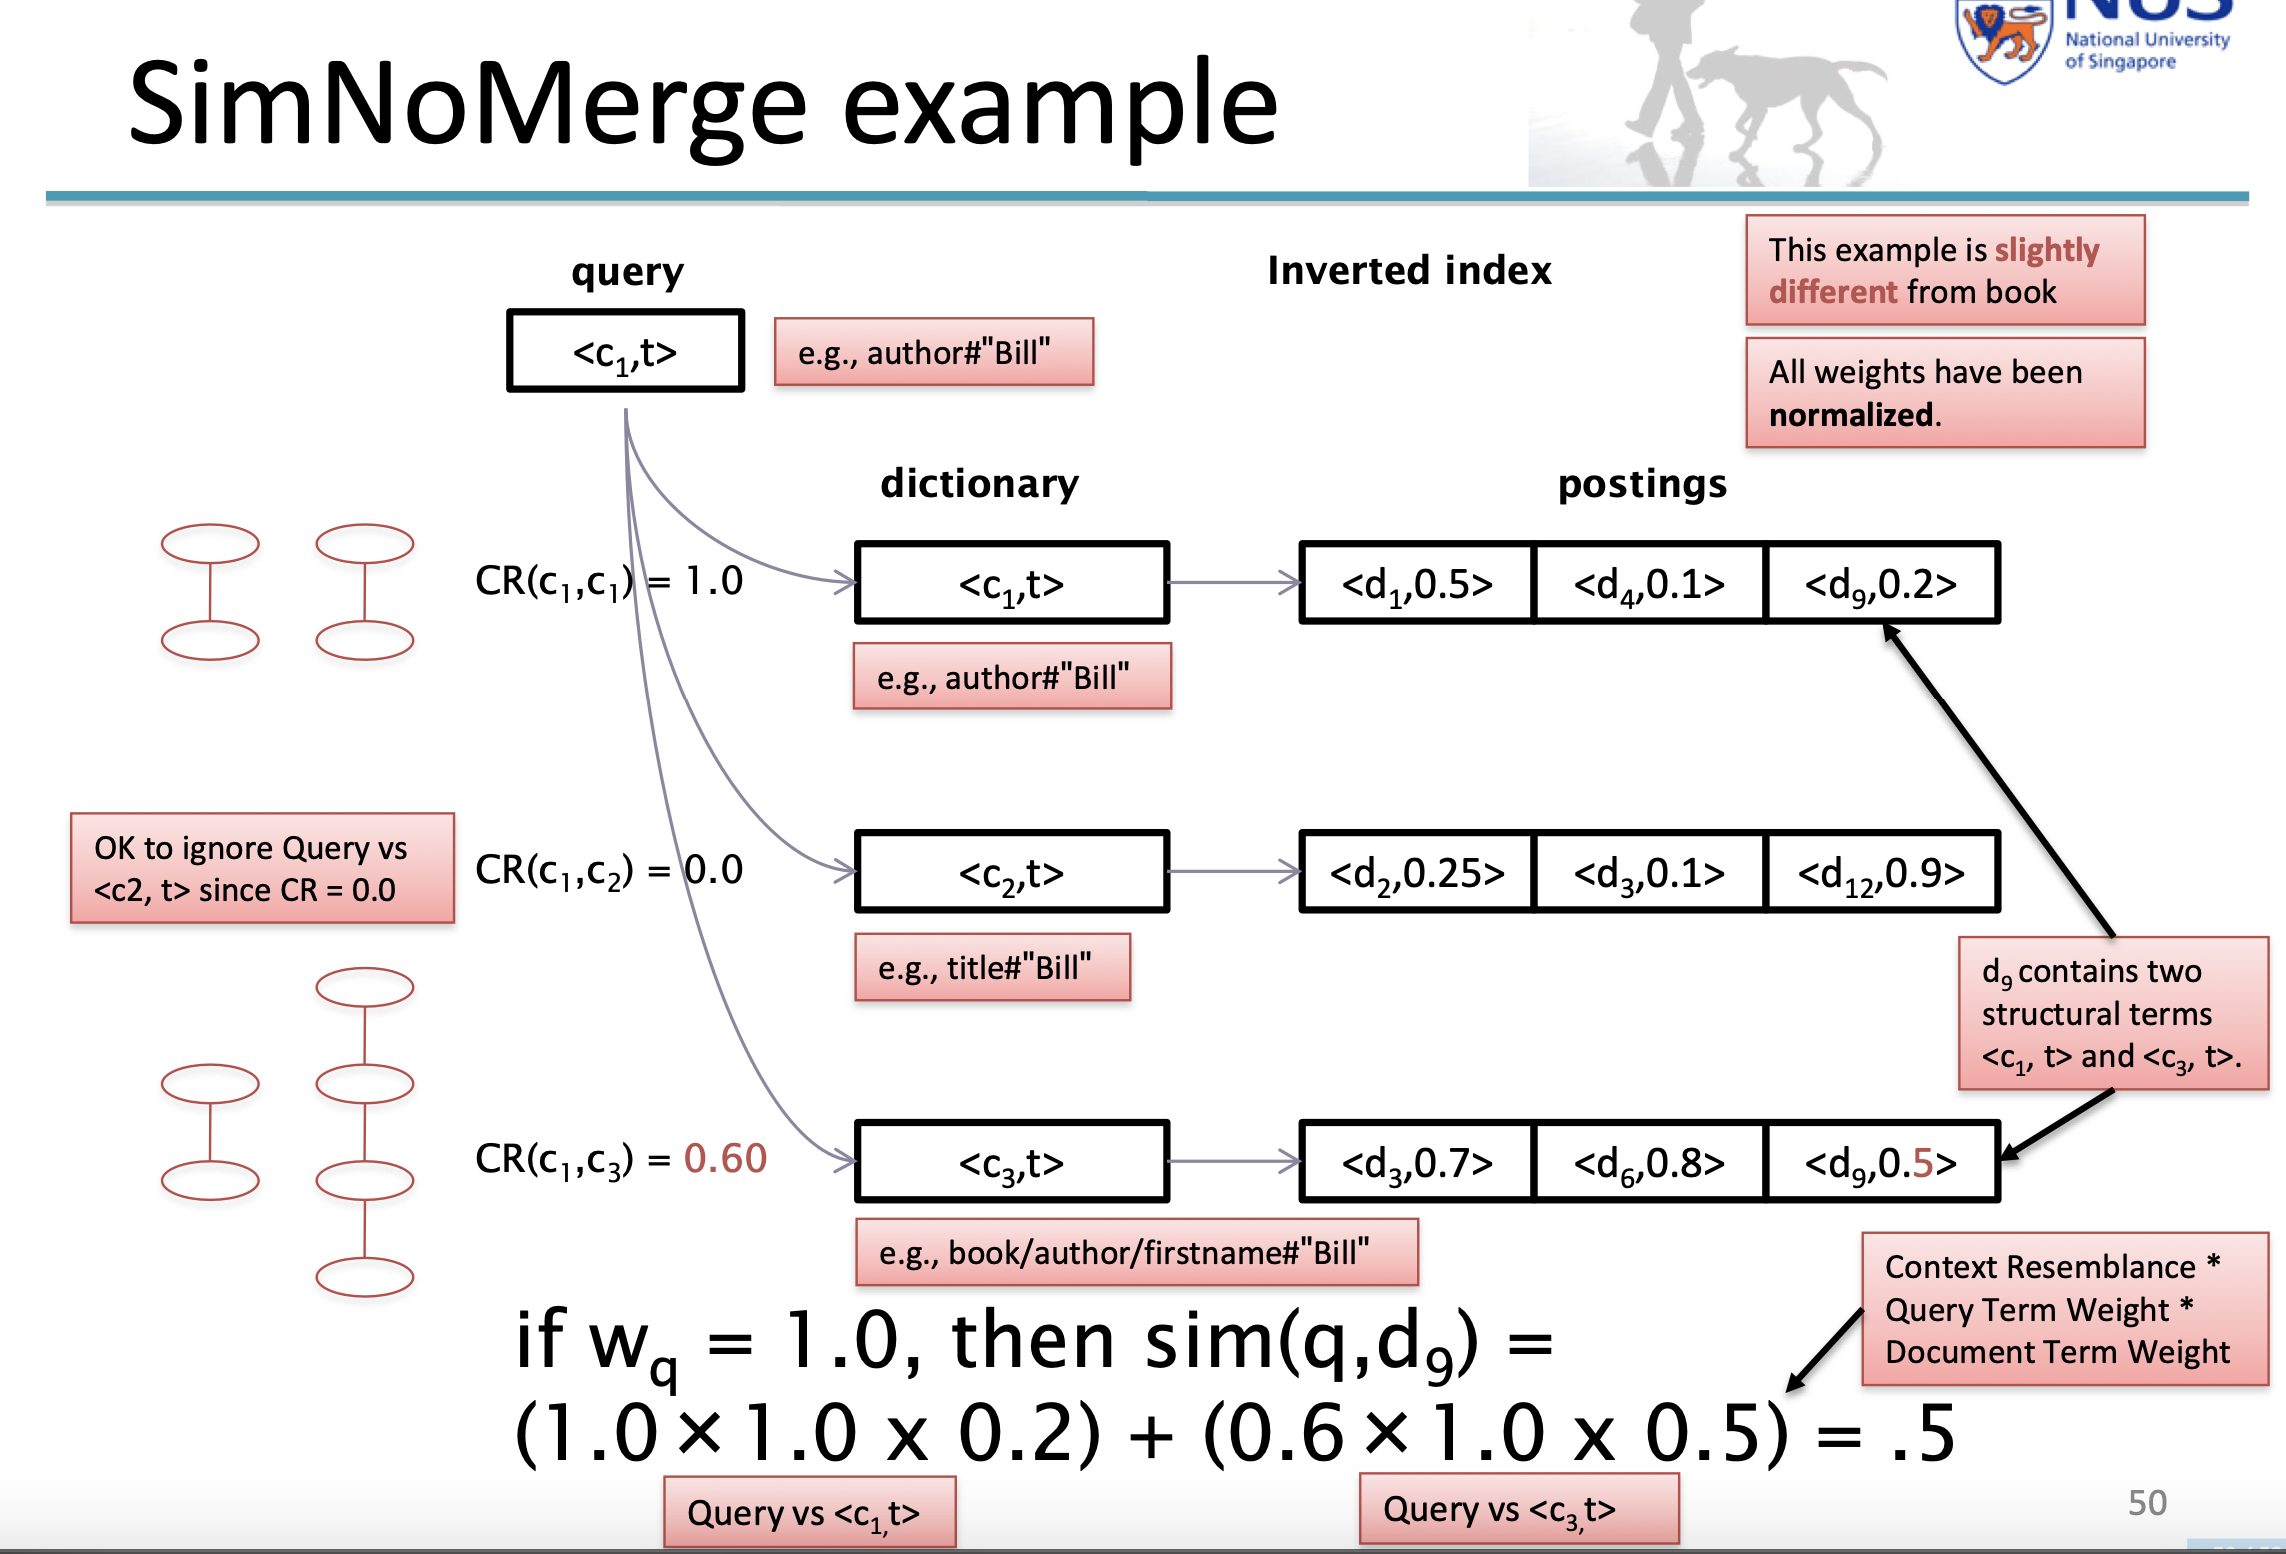
\includegraphics[height=7cm]{ir18}\\
Cr(c1, c3) = 1 + 2 / 1 + 4 = 0.60
\\
Check if there are duplicates in structural terms 
\subsection*{Link analysis - Pagerank}
Damping factor 0.9 (10\% teleportation rate)\\\\
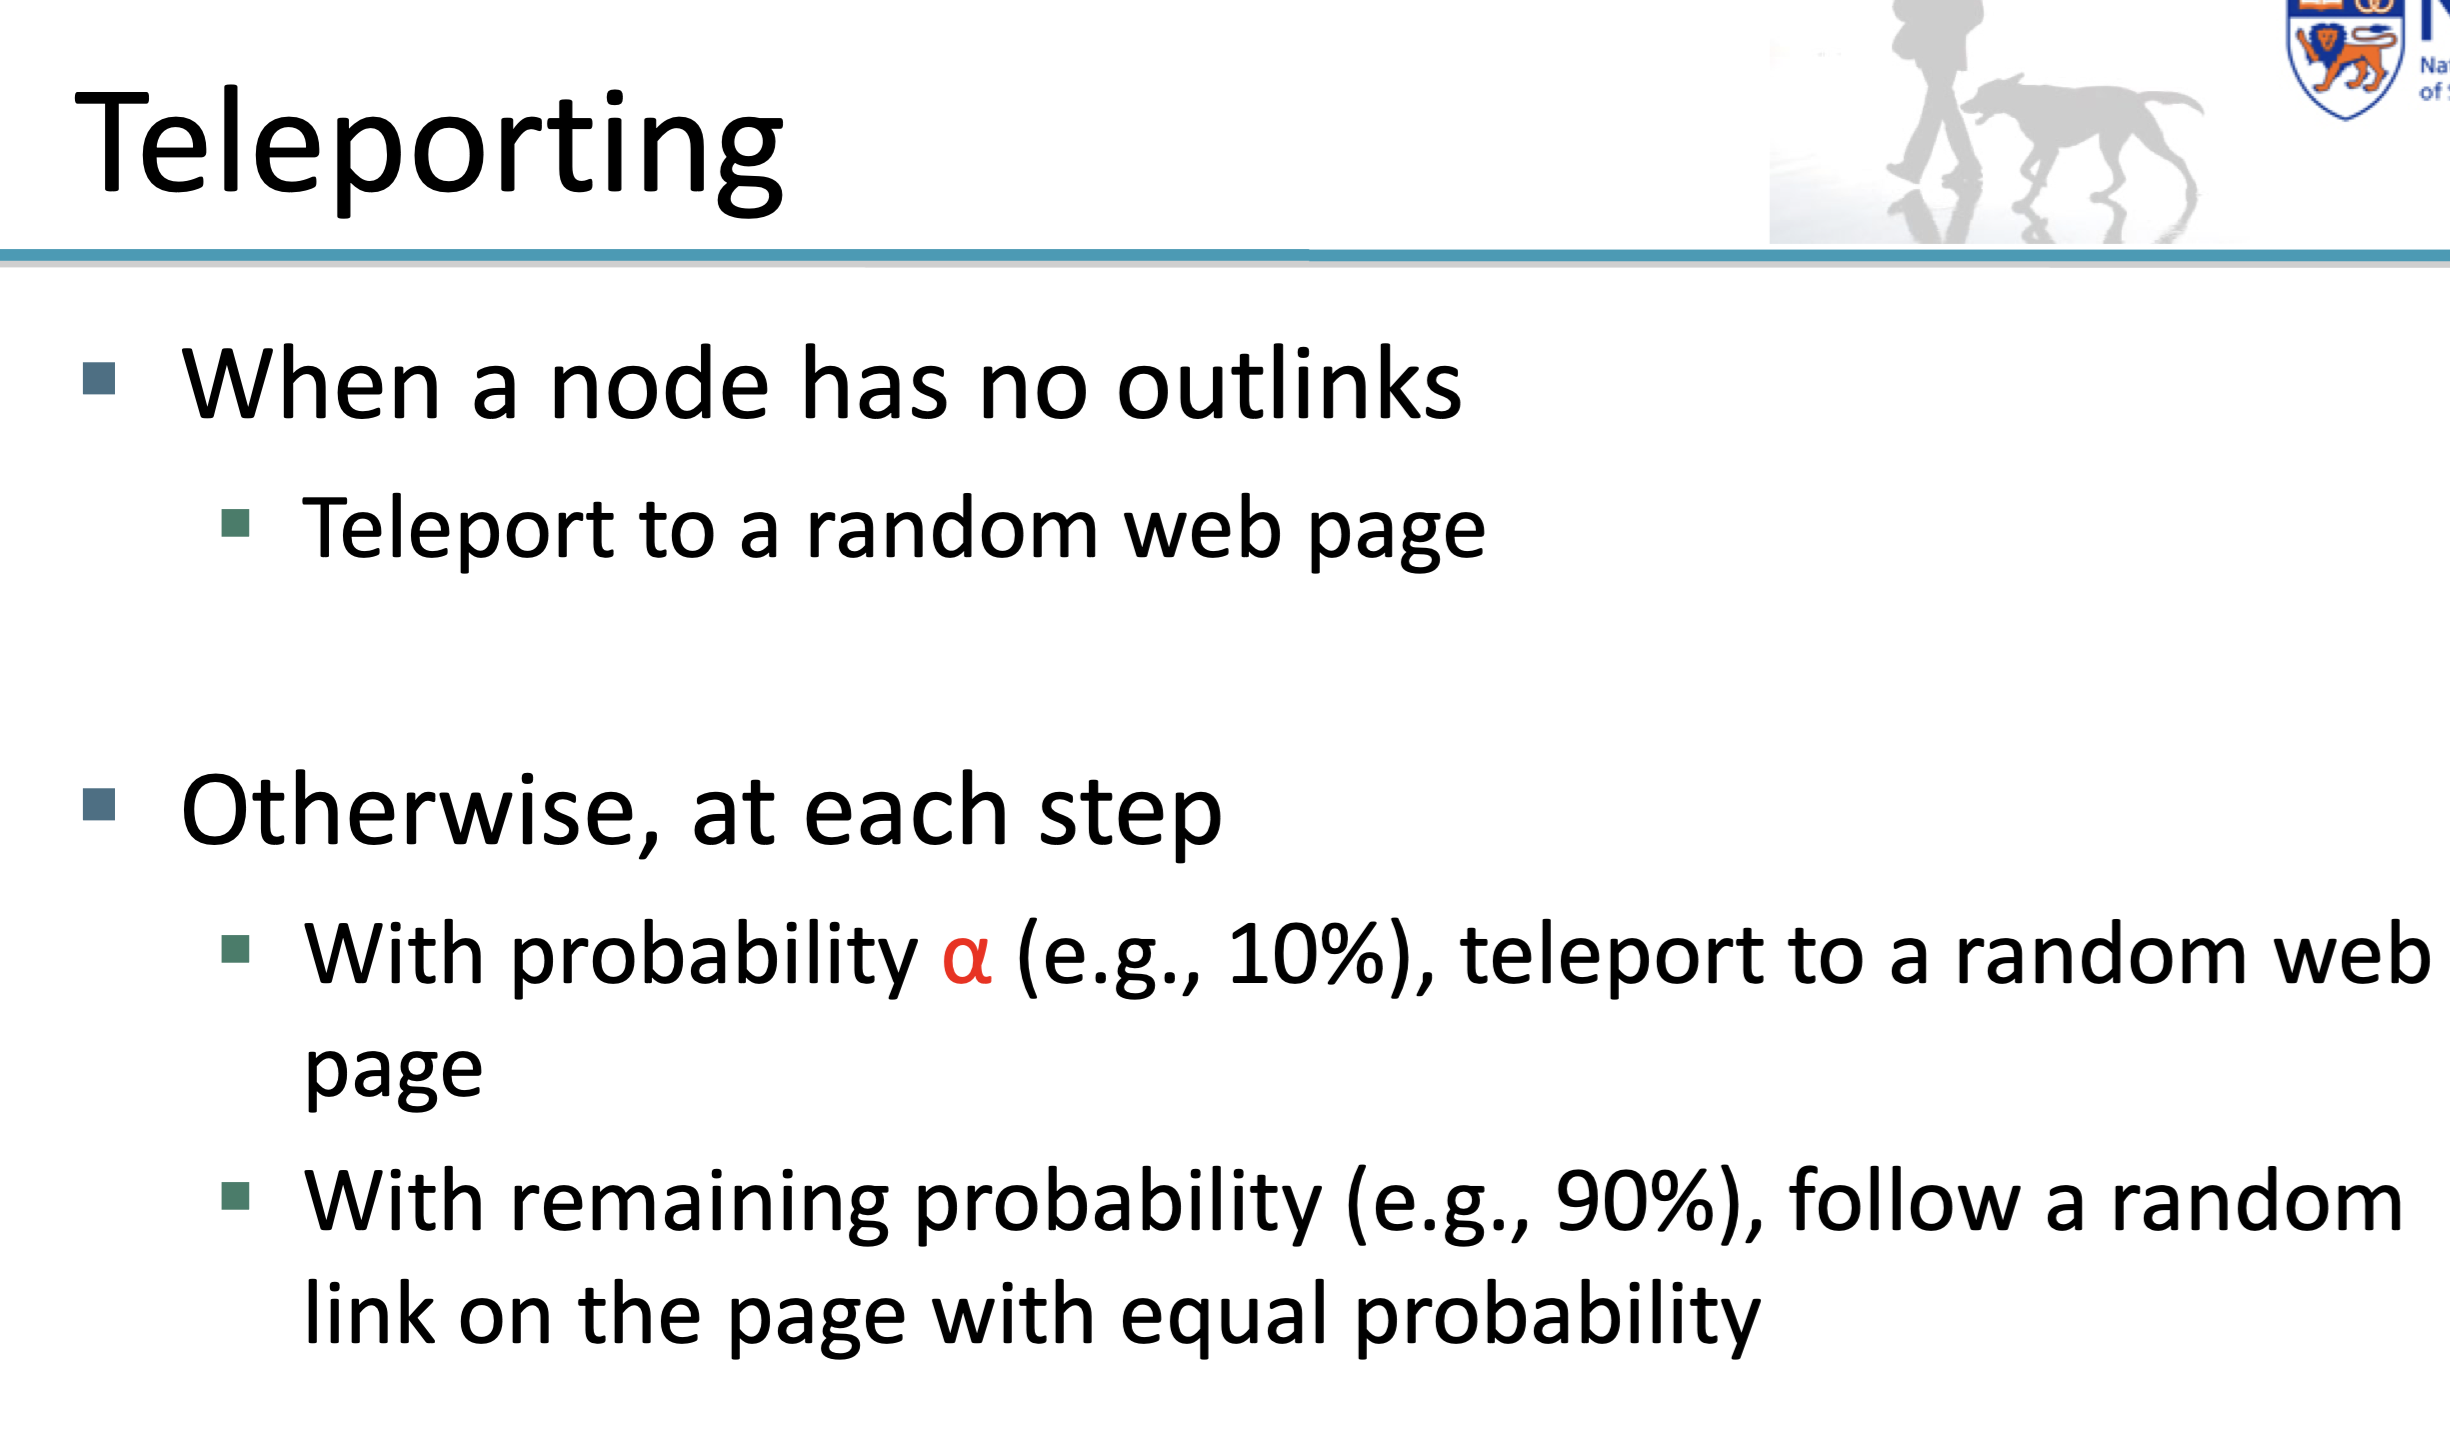
\includegraphics[height=5cm]{ir16}
\\
To get nth iteration, multiply [1/n ... 1/n] with the power of the matrix 
\end{multicols*}

\end{document}
